\usepackage{graphicx}
\usepackage{verbatim}
\usepackage{latexsym}
\usepackage{mathchars}
\usepackage{setspace}
\usepackage[toc]{appendix}
%neu hinzu
\usepackage{subcaption}
\usepackage{extarrows}
\usepackage{nicefrac}
\usepackage[ngerman]{babel}
\usepackage{amsthm}
\usepackage{amsmath,amsfonts,amssymb}
\usepackage{bm}
\usepackage{dsfont}
\usepackage{multirow}
% package minted for code-snippets
\usepackage{listings}
\usepackage{xcolor}
%\usepackage{appendix}
\usepackage{natbib} %[round,comma,authoryear]
\bibliographystyle{humannat}
% styles: "plain","unsrt","alpha",

\input{blocked.sty}
\input{uhead.sty}
\input{boxit.sty}
\documentclass[a4paper,12pt,twoside]{report}
\usepackage[left=2.5cm,right=2.5cm,top=2cm,bottom=3cm]{geometry}

\usepackage{graphicx}
\usepackage{verbatim}
\usepackage{latexsym}
\usepackage{mathchars}
\usepackage{setspace}
\usepackage[toc]{appendix}
%neu hinzu
\usepackage{subcaption}
\usepackage{extarrows}
\usepackage{nicefrac}
\usepackage[ngerman]{babel}
\usepackage{amsthm}
\usepackage{amsmath,amsfonts,amssymb}
\usepackage{bm}
\usepackage{dsfont}
\usepackage{multirow}
% package minted for code-snippets
\usepackage{listings}
\usepackage{xcolor}
%\usepackage{appendix}
\usepackage{natbib} %[round,comma,authoryear]
\bibliographystyle{humannat}
% styles: "plain","unsrt","alpha",

\input{blocked.sty}
\input{uhead.sty}
\input{boxit.sty}
\documentclass[a4paper,12pt,twoside]{report}
\usepackage[left=2.5cm,right=2.5cm,top=2cm,bottom=3cm]{geometry}

\include{thesis.preamble}


\begin{document}

\title{Your Thesis Title}

\author{Falko Krause Cauduro}
\submitdate{May 2020}
\degree{BSc Wirtschaftsmathematik}
\studentid{2714676}
\supervisor{Prof. Dr. rer. nat. habil. Ralf Wunderlich}

\normallinespacing
\maketitle

% delete the two declaration sentences in thesis.sty if not applicable. 

\preface
\input{abstract/abstract}
\input{acknowledgements/acknowledgements}

% There is a maximum limit of 15,000 words without exceeding 40 pages (A4 sides) for the main body of the dissertation that will be submitted in PDF. This limitation includes the bibliography and excludes cover/front pages (e.g., abstract, acknowledgement, table of contents) and excludes the appendices, listing of any codes or any other supporting documentation.
% Note: Your dissertation should not exceed the word and page limits. You do not have to use up your word limit to get a good grade; never `pad out' your dissertation, this will only annoy the markers.

\body
\include{introduction/introduction}
\include{background/background}

% body of thesis comes here
\input{body/body}

\include{summary/summary}

% Bibliography
\addcontentsline{toc}{chapter}{Bibliography}
%\bibliographystyle{alpha}
\bibliography{bibliography/bibliography}




% appendices come here

\input{appendices/appendices}


\end{document}

\newcommand{\ipc}{{\sf ipc}}

\newcommand{\Prob}{\bbbp}
\newcommand{\Real}{\bbbr}
\newcommand{\real}{\Real}
\newcommand{\Int}{\bbbz}
\newcommand{\Nat}{\bbbn}

\newcommand{\NN}{{\sf I\kern-0.14emN}}   % Natural numbers
\newcommand{\ZZ}{{\sf Z\kern-0.45emZ}}   % Integers
\newcommand{\QQQ}{{\sf C\kern-0.48emQ}}   % Rational numbers
\newcommand{\RR}{{\sf I\kern-0.14emR}}   % Real numbers
\newcommand{\KK}{{\cal K}}
\newcommand{\OO}{{\cal O}}
\newcommand{\AAA}{{\bf A}}
\newcommand{\HH}{{\bf H}}
\newcommand{\II}{{\bf I}}
\newcommand{\LL}{{\bf L}}
\newcommand{\PP}{{\bf P}}
\newcommand{\PPprime}{{\bf P'}}
\newcommand{\QQ}{{\bf Q}}
\newcommand{\UU}{{\bf U}}
\newcommand{\UUprime}{{\bf U'}}
\newcommand{\zzero}{{\bf 0}}
\newcommand{\ppi}{\mbox{\boldmath $\pi$}}
\newcommand{\aalph}{\mbox{\boldmath $\alpha$}}
\newcommand{\bb}{{\bf b}}
\newcommand{\ee}{{\bf e}}
\newcommand{\mmu}{\mbox{\boldmath $\mu$}}
\newcommand{\vv}{{\bf v}}
\newcommand{\xx}{{\bf x}}
\newcommand{\yy}{{\bf y}}
\newcommand{\zz}{{\bf z}}
\newcommand{\oomeg}{\mbox{\boldmath $\omega$}}
\newcommand{\res}{{\bf res}}
\newcommand{\cchi}{{\mbox{\raisebox{.4ex}{$\chi$}}}}
%\newcommand{\cchi}{{\cal X}}
%\newcommand{\cchi}{\mbox{\Large $\chi$}}

% Logical operators and symbols
\newcommand{\imply}{\Rightarrow}
\newcommand{\bimply}{\Leftrightarrow}
\newcommand{\union}{\cup}
\newcommand{\intersect}{\cap}
\newcommand{\boolor}{\vee}
\newcommand{\booland}{\wedge}
\newcommand{\boolimply}{\imply}
\newcommand{\boolbimply}{\bimply}
\newcommand{\boolnot}{\neg}
\newcommand{\boolsat}{\!\models}
\newcommand{\boolnsat}{\!\not\models}


\newcommand{\op}[1]{\mathrm{#1}}
\newcommand{\s}[1]{\ensuremath{\mathcal #1}}

% Properly styled differentiation and integration operators
\newcommand{\diff}[1]{\mathrm{\frac{d}{d\mathit{#1}}}}
\newcommand{\diffII}[1]{\mathrm{\frac{d^2}{d\mathit{#1}^2}}}
\newcommand{\intg}[4]{\int_{#3}^{#4} #1 \, \mathrm{d}#2}
\newcommand{\intgd}[4]{\int\!\!\!\!\int_{#4} #1 \, \mathrm{d}#2 \, \mathrm{d}#3}

% Large () brackets on different lines of an eqnarray environment
\newcommand{\Leftbrace}[1]{\left(\raisebox{0mm}[#1][#1]{}\right.}
\newcommand{\Rightbrace}[1]{\left.\raisebox{0mm}[#1][#1]{}\right)}

% Funky symobols for footnotes
\newcommand{\symbolfootnote}{\renewcommand{\thefootnote}{\fnsymbol{footnote}}}
% now add \symbolfootnote to the beginning of the document...

\newcommand{\normallinespacing}{\renewcommand{\baselinestretch}{1.5} \normalsize}
\newcommand{\mediumlinespacing}{\renewcommand{\baselinestretch}{1.2} \normalsize}
\newcommand{\narrowlinespacing}{\renewcommand{\baselinestretch}{1.0} \normalsize}
\newcommand{\bump}{\noalign{\vspace*{\doublerulesep}}}
\newcommand{\cell}{\multicolumn{1}{}{}}
\newcommand{\spann}{\mbox{span}}
\newcommand{\diagg}{\mbox{diag}}
\newcommand{\modd}{\mbox{mod}}
\newcommand{\minn}{\mbox{min}}
\newcommand{\andd}{\mbox{and}}
\newcommand{\forr}{\mbox{for}}
\newcommand{\EE}{\mbox{E}}

\newcommand{\deff}{\stackrel{\mathrm{def}}{=}}
\newcommand{\syncc}{~\stackrel{\textstyle \rhd\kern-0.57em\lhd}{\scriptstyle L}~}

\def\coop{\mbox{\large $\rhd\!\!\!\lhd$}}
\newcommand{\sync}[1]{\raisebox{-1.0ex}{$\;\stackrel{\coop}{\scriptscriptstyle
#1}\,$}}


% 1. format for definition-equality ":=" via \defeq
\makeatletter
\newcommand*{\defeq}{\mathrel{\vcenter{\baselineskip0.5ex \lineskiplimit0pt
                     \hbox{\scriptsize.}\hbox{\scriptsize.}}}%
                     =}
\makeatother

% 2. format for definition-equality ":=" via := (kann eigentlich weg, da 1. Format reicht)
\mathchardef\ordinarycolon\mathcode`\:
\mathcode`\:=\string"8000
\begingroup \catcode`\:=\active
  \gdef:{\mathrel{\mathop\ordinarycolon}}
\endgroup


% define new theoremstyle for algorithm headers
\newtheoremstyle{algodd} % name of the style to be used
  {} % measure of space to leave above the theorem. E.g.: 3pt oder \topsep
  {} % measure of space to leave below the theorem. E.g.: 3pt
  {\upshape} % name of font to use in the body of the theorem, e.g. \itshape for italic oder \em
  {8pt}     % measure of space to indent e.g. \parindent oder "8pt"
  {\bfseries} % name of head font, e.g. \bfseries oder \bf
  {}    % punctuation after theorem head -> between head and body
  {\newline} % space after theorem head; { } = normal interword space {\newline} = linebreak, {.5em} = Half the size of Letter M?
  {\thmname{#1}\thmnumber{ #2}:\thmnote{ #3}} %headspec, empty=normal, hier note field in Bold, Sollen die Klammern weg, dann am Ende "(#3)" statt "#3" setzen.
% {\thmname{#1}\thmnumber{\addtocounter{thm}{-1} #2$^\prime$}\thmnote{\textnormal{ (#3)}}}

% define new theoremstyle for bold definition headers
\newtheoremstyle{theoremdd} % name of the style to be used
  {} % measure of space to leave above the theorem. E.g.: 3pt oder \topsep
  {} % measure of space to leave below the theorem. E.g.: 3pt
  {\upshape} % name of font to use in the body of the theorem, e.g. \itshape for italic oder \em
  {16pt}     % measure of space to indent e.g. \parindent oder "8pt"
  {\bfseries} % name of head font, e.g. \bfseries oder \bf
  {:}    % punctuation after theorem head -> between head and body
  { }      % space after theorem head; { } = normal interword space {\newline} = linebreak, {.5em} = Half the size of Letter M?
  {\thmname{#1}\thmnumber{ #2}\thmnote{ (#3)}} %headspec, empty=normal, hier note field in Bold, Sollen die Klammern weg, dann am Ende "#3" statt "(#3)" setzen.
% {\thmname{#1}\thmnumber{\addtocounter{thm}{-1} #2$^\prime$}\thmnote{\textnormal{ (#3)}}}


\theoremstyle{theoremdd}
%\theoremstyle{definition} % mit "definition" wäre es klassischer style 
\newtheorem{definition}{Def.}[subsection]
% Bsp. sollen gleichen Zähler haben wie Def., daher "[definition]" in der Mitte statt "[subsection]" am Ende zu deklarieren, dann hätten Bsp. eigenen Counter
% auch den style "definition" teilen sich Bsp. mit den Def.
\newtheorem{example}[definition]{Bsp.}
% Bemerkungen nicht nummeriert
\newtheorem*{remark}{Bem.}

\theoremstyle{algodd}
\newtheorem{algorithm}{Algorithmus}[chapter]

\theoremstyle{plain} % "plain" = kursiver Text
\newtheorem{theorem}{Satz}[chapter]
% the counter of this new environment will be reset every time a new theorem environment is used
\newtheorem{corollary}{Korollar}[theorem]
% same counter as theorems
\newtheorem{lemma}[theorem]{Lemma}


\newcommand{\Figref}[1]{Figure~\ref{#1}}
\newcommand{\fig}[3]{
 \begin{figure}[!ht]
 \begin{center}
 \scalebox{#3}{\includegraphics{figs/#1.ps}}
 \vspace{-0.1in}
 \caption[ ]{\label{#1} #2}
 \end{center}
 \end{figure}
}

\newcommand{\figtwo}[8]{
 \begin{figure}
 \parbox[b]{#4 \textwidth}{
 \begin{center}
 \scalebox{#3}{\includegraphics{figs/#1.ps}}
 \vspace{-0.1in}
 \caption{\label{#1}#2}
 \end{center}
 }
 \hfill
 \parbox[b]{#8 \textwidth}{
 \begin{center}
 \scalebox{#7}{\includegraphics{figs/#5.ps}}
 \vspace{-0.1in}
 \caption{\label{#5}#6}
 \end{center}
 }
 \end{figure}
}

% for codesnippets
\definecolor{codegreen}{rgb}{0,0.6,0}
\definecolor{codegray}{rgb}{0.5,0.5,0.5}
\definecolor{codepurple}{rgb}{0.58,0,0.82}
\definecolor{backcolour}{rgb}{0.95,0.95,0.92}

\lstdefinestyle{mystyle}{
    backgroundcolor=\color{backcolour},   
    commentstyle=\color{codegreen},
    %keywordstyle=\color{magenta},
    numberstyle=\tiny\color{codegray},
    %stringstyle=\color{codepurple},
    basicstyle=\ttfamily\footnotesize,
    breakatwhitespace=false,         
    breaklines=true,                 
    captionpos=b,                    
    keepspaces=true,                 
    numbers=left,                    
    numbersep=5pt,                  
    showspaces=false,                
    showstringspaces=false,
    showtabs=false,                  
    tabsize=2
}

\lstset{style=mystyle}


\begin{document}

\title{Your Thesis Title}

\author{Falko Krause Cauduro}
\submitdate{May 2020}
\degree{BSc Wirtschaftsmathematik}
\studentid{2714676}
\supervisor{Prof. Dr. rer. nat. habil. Ralf Wunderlich}

\normallinespacing
\maketitle

% delete the two declaration sentences in thesis.sty if not applicable. 

\preface
\addcontentsline{toc}{chapter}{Abstract}



    \begin{quotation}
        \glqq […] \textit{Since all models are wrong the scientist cannot obtain a ``correct'' one by excessive elaboration. 
        On the contrary, following William of Occam he should seek an economical description of natural phenomena. 
        Just as the ability to devise simple but evocative models is the signature of the great scientist 
        so overelaboration and overparameterization is often the mark of mediocrity.}\grqq{} George E.P. Box, 1976
    \end{quotation}


\begin{abstract}

Es werden zunächst klassische Konzentrations- und Entropiemaße der deskriptiven räumlichen Statistik angewandt.
Darauf folgt die Anwendung einer Clusteranalyse durch globale Indizes (Moran’s I und Geary’s c)
und statistischer Tests auf Signifikanz, 
sowie spezialisierter lokaler Maße und Tests (Local Getis GI, Local Morans’ I). 
Daran knüpfen räumliche Regressionsmodelle an, deren Parameter durch Inferenzverfahren ermittelt werden.\\


\end{abstract}


\textbf{Erklärung}

Der Verfasser erklärt, dass er die vorliegende Arbeit selbständig, ohne fremde Hilfe und ohne Benutzung anderer 
als der angegebenen Hilfsmittel angefertigt hat. Die aus fremden Quellen (einschließlich elektronischer Quellen) 
direkt oder indirekt übernommenen Gedanken sind ausnahmslos als solche kenntlich gemacht. 
Wörtlich und inhaltlich verwendete Quellen wurden entsprechend den anerkannten Regeln wissenschaftlichen Arbeitens zitiert. 
Die Arbeit ist nicht in gleicher oder vergleichbarer Form, auch nicht  auszugsweise im Rahmen einer anderen Prüfung 
bei  einer anderen Hochschule vorgelegt worden.\\

Sie wurde bisher auch nicht veröffentlicht.\\

Ich erkläre mich damit einverstanden, dass die Arbeit mit Hilfe eines Plagiatserkennungsdienstes auf enthaltene Plagiate überprüft wird.\\
\\


Ort, Datum       $\qquad \qquad$           Unterschrift des Verfassers     
\cleardoublepage

\addcontentsline{toc}{chapter}{Danksagung} %engl.: "Acknowledgements"

\begin{acknowledgements}


Auf diesem Wege danke ich all jenen Personen, die mich während der Arbeiten an diesem umfangreichen Thema unterstützt haben. \\

Besonderer Dank gilt hierbei meinem Betreuer Herrn Prof. Dr. Ralf Wunderlich, der mir mit Rat und Fachwissen stets zur Seite steht 
sowie Herrn Prof. Dr. Carsten Hartmann für das bereitwillige Teilen seines Wissensschatzes und seiner Erfahrung. 
Ich schätze mich äußerst glücklich, von beiden Persönlichkeiten zu lernen. \\

Ganz besonders danke ich meiner Familie für ihre unbedingte Unterstützung und all die Energie und Inspiration.





\end{acknowledgements}

% There is a maximum limit of 15,000 words without exceeding 40 pages (A4 sides) for the main body of the dissertation that will be submitted in PDF. This limitation includes the bibliography and excludes cover/front pages (e.g., abstract, acknowledgement, table of contents) and excludes the appendices, listing of any codes or any other supporting documentation.
% Note: Your dissertation should not exceed the word and page limits. You do not have to use up your word limit to get a good grade; never `pad out' your dissertation, this will only annoy the markers.

\body
\chapter{Einführung} %engl. "Introduction"

A good proportion of the data out there in the real world is inherently spatial. 
From the population recorded in the national census, to every shop in your neighborhood, 
the majority of datasets have a location aspect that you can exploit to make the most of what they have to offer.

You will then combine different sources using their location as the bridge that puts them in relation to each other, allowing you to transform and repurpose them in different contexts.

Quantitative Revolution der Geographie?

Setting out the aims and objectives of your project, explaining the overall intention of the project and specific steps that will be taken to achieve that intention.

\section{Motivation}

Explaining the problem being solved.


\section{Aims and Objectives}

Ziele und Vorgaben der Arbeit.

Als Bachelorarbeit liegt die Absicht in einer möglichst breiten Aufgliederung vieler Aspekte, ohne (im Gegensatz zu einem Handbuch) Details und tiefere Analyse leisten zu können.  
Der Fokus liegt auf einer schnell und einfach lesbaren Aufbereitung der Grundlagen räumlicher Statistik mit einer groben Einteilung der größten Teilgebiete, 
sodass dem Leser eine schnelle und effiziente Übersicht über einen großen Forschungszweig zur eigenen Orientierung gegeben wird.

Zugleich wird die Anwendung auf ein spezielles Thema einen beispielhaften Einblick in den Prozess einer Modellbildung und die Pipeline der Datenanalyse 
zur Orientierung geliefert.

Dieser Spagat zwischen theoretischer Abstrahierung und praktischer Anwendung soll ein Gefühl der Anwendbarkeit und Relevanz vermitteln und die Bandbreite verdeutlichen.


\section{Description of the work}

Explaining what your project is meant to achieve, how it is meant to function, perhaps even a functional specification.



\chapter{Background and Related Work}\label{ch:background} 

Explaining what your project does that is new or is better than existing work in the same field.

%Test citation \cite{cormen2009introduction}.
\section{GIS Details}

Fischer Getis 2010, S. 55 

Spatial Data in R
\section{Quellen und Literatur}

Tabelle XX liefert eine Auflistung der Standardwerke und Handbücher, wie sie auch in diese Arbeit eingeflossen sind.

% body of thesis comes here
\chapter{Datentypen und Methodenklassen}

%\section{Einleitung}

räumlich (gebietlichen, regionalen, lokalen, örtlich, mehrdimensionalen, Raumordnung, Lagebeziehung, Raum-, Orts-, Lage-, Flächen-) \\

räumlich verteilte Positionen (Standorte, Lokationen, Stellen, Lageparameter) \\
diskrete Raumzonen \\

an Positionen beobachtete Daten (Ausprägungen, Zielwerte, Attributsrealisierung) 

\section{Besonderheiten räumlicher Daten}

\subsection*{Räumliche Assoziation?}
\label{subsec:tobler}

Abbildung \ref{fig_densitymaps} verdeutlicht das Konzept räumlicher Autokorrelation. Die starke Präsenz von räumlicher 
Abhängigkeit verkompliziert die Analyse, da nicht von unabhängigen Daten ausgegangen werden kann. Abb 3.2 zeigt grob auf,
welches Erscheinungsbild eine (über Verwaltungskreise) zufällig verteilte Bevölkerung aufwiese.

\begin{figure} %[htb] %h=here, t=top, b=bottom, p=page of float
    \centering %Bilder mittig statt am linken Rand ausgerichtet
    \begin{minipage}[b]{.45\linewidth} % [b] => Ausrichtung an \caption --> c (=Center) t (=Top) und b (=Bottom)
        % \linewidth entspricht hier \textwidth (=Breite Textbereich)
        %\centering
        %                                 trim = links unten rechts oben
        \includegraphics[width=\linewidth,trim={2cm 1cm 1cm 1cm},clip]{body/figures/popdens2018.pdf} % [scale=0.5] oder [width=\linewidth]
       %\includegraphics[scale=0.4,trim={1cm 2cm 1cm 2cm},clip]{body/figures/popdens2018.pdf} % [scale=0.5] oder [width=\linewidth]
       %[width=\textwidth] entspricht [width=\linewidth] (=Breite einer Minipage)
       \caption{reale Daten}
    \end{minipage} % <- sonst wird hier ein Leerzeichen eingefügt
    \hfill
    %\hspace{.1\linewidth}% Abstand zwischen Bilder
    \begin{minipage}[b]{.45\linewidth}
        %\centering
       \includegraphics[width=\linewidth,trim={2cm 1cm 1cm 1cm},clip]{body/figures/popdens2018-rdm.pdf}
       \caption{randomisierte Daten}
    \end{minipage}
    \caption[Bevölkerungsdichten ]{Autokorrelation der Bevölkerungsdichte je Kreis in 2018. Grafik erstellt mit Daten aus: Quelle}
    \label{fig_densitymaps}
 \end{figure}

Hier besteht die Annahme, dass räumlich benachbarte Beobachtungen einer Variablen/Attributs ähnlicher 
sind als weit entfernte. Dieser Umstand wird durch Toblers erstes Gesetz der Geographie 
ausgedrückt \cite[S.234]{tobler_computer_1970}:
\begin{quotation}
    \glqq […] \textit{the first law of geography: everything is related to everything else, 
    but near things are more related than distant things.}\grqq{} Waldo R. Tobler
\end{quotation}
Trotz ihrer simplen Präsentation und obwohl diese Formulierung eher wie 
common sense anmuted und fraglich ist, ob tatsächlich 
\glqq alles miteinander in Beziehung steht\grqq{} wie \cite{tobler_first_2004} selbst anmerkt, 
so ist er der erste Wissenschaftler, der dieses grundlegende Konzept 
räumlicher Dynamik klar ausformulierte. \newline
Inwiefern zwischen einem universalen wissenschaftliches Gesetz und einer beobachteten 
Regelmäßigkeit (engl. causality vs regularity) unterschieden werden kann und ob in 
den Sozialwissenschaften von Gesetzen gesprochen werden kann, ist Gegenstand 
wissenschaftlicher Auseinandersetzung (e.g. Law of Utility Maximization) \cite{goodchild_validity_2004}. 
Tobler argumentiert mit der Distanz als Ursache und argumentiert somit gegen die Sicht, 
dass Distanz und räumliche Verteilung von Merkmalen als zwei Beobachtungen einer 
verborgenen Ursache nur „beobachtete Regelmäßigkeiten“ sind. (Verweis auf Feynman?) \cite{sui_toblers_2004} 
%Block eher in die Einleitung?
Die Theorie fällt historisch in die Zeit der Quantitativen Revolution der 
modernen Geographie (s. Kapitel1?), wird jedoch erst mit Aufkommen und Verbreitung 
geographischer Informationssysteme (GIS) seit den 1990er Jahren in größerem Umfang 
beachtet, gelehrt und referenziert [Sui-Forum].
%Ende

Das Gesetz entspricht der menschlichen Intuition aus historischen 
Beobachtungen und ist fest verankert in wissenschaftlichen Paradigmen. 
In der Theorie basiert diese Gesetzmäßigkeit wiederum auf dem Konzept 
der \emph{Distanzreibung} (engl. friction of distance) 
und daraus resultierenden Abklingfunktionen (engl. distance decay) für allgemeine räumliche Merkmale. 
Derartige Abklingfunktionen bilden die Grundlage für die Interpolationsmethoden der \emph{Geostatistik}, 
wie in Kapitel \ref{subsec:geostatistics} näher erläutert wird.
Weitere Grundlage räumlicher Interpolation ist die Messung der Ähnlichkeit räumlich benachbarter Merkmale 
als Ziel der Theorie \emph{räumlicher Autokorrelation} (engl. spatial autocorrelation). 
%Abschnitt in Autokorrelationskapitel rein
Die räumliche Lage/Position einer Punktmessung liefert selbst bereits implizit inhärente Zusatzinformationen 
über die Beobachtungswerte in der Umgebung des Beobachtungswertes. 
Diese Autokorrelation stört somit die Grundannahme einer \emph{unabhängig identisch verteilten} (i.i.d.) Grundgesamtheit, 
da Messungen an verschiedenen Positionen nicht unabhängig voneinander sind, insbesondere bei geringer Distanz zueinander. 
%Abschnitt-Ende
In Kapitel \ref{ch:autocorrelation} werden globale und lokale Autokorrelationsindikatoren zur 
Detektion räumlich-zeitlicher hot- und coldspots und als Werkzeuge der Regression eingeführt.

Zunehmende Distanz erhöht zudem die Kosten der Interaktion zwischen Raumpunkten. 
Im Beispiel der sozio-ökonimschen Gravitationsmodelle beeinflussen 
der (teilweise in Transportkosten enthaltene) Energie-, Zeit und Materialaufwand für Mobilität  
die kulturelle, soziale und politisch-wirtschaftliche Distanz.
Die Distanzreibung dient zudem der Erklärung historischer Wirtschaftsentwicklung, 
militärischer Dominanz eines Staates 
bis hin zu ökologischen Ausbreitungsmustern von Vegetationszonen und Tierarten. 
Das geografische Gesetz begründet auf Grundlage dieser Distanzeffekte die Beobachtung annähernd 
homogener Regionen und zusammenhängende Gebiete mit 
ähnlichen Merkmalen (e.g. Städte, Vegetationszonen, Planetensysteme? Usw.).

Geringere Bekanntheit erlangte Toblers zweites Gesetz: 
\glqq\textit{The phenomenon external to an area 
of interest affects what goes on inside}\grqq{}.
Hiermit weist er darauf hin, dass in praktischen Experimenten die Abmessungen des endlichen 
Beobachtungsraumes zu einem bestimmten Grad willkürlich gewählt sind und weiterhin durch Vorgänge über 
die Abgrenzung hinaus beeinflusst werden. 
Viele Phänomen weisen Autokorrelationen zwischen räumlichen Zonen auf, (welche nicht im untersuchten Prozess begründet liegt?).
Problematisch ist die fehlende Unabhängigkeit der Stichproben aufgrund der räumlichen Nähe. 
Eine Auseinandersetzung ist 1889 als "Galtons Problem" überliefert, in welcher Sir Francis Galton auf Fehlschlüsse hinweist, sobald Daten nicht mehr unabhängig voneinander sind.
Er zeigte, dass positive räumliche Abhängigkeit den Informationsgehalt der Beobachtungen verringert, 
da sie durch andere Beobachtungen in der Nähe teilweise prognostiziert werden können. 
Dies reduziert den effektiven Stichprobenumfang. In solch einem Fall liegt den abhängigen Daten ein gemeinsamer Vorgang zugrunde, 
während eine räumliche Aufteilung in verschiedene Zonen voneinander unabhängige Daten suggeriert/vorgaukelt (Bivand S. 264).

Im folgenden Abschnitt wird auf weitere Probleme der Zerlegung und Skalierung eingegangen.

\subsection*{Räumliche Aggregationseffekte}
Beobachtungsmerkmale können durch Skalierung ihr Verhalten/Gesetzmäßigkeiten ändern. 
So lässt sich die Länge einer Küstenlinie nicht eindeutig bestimmen, sondern wird aufgrund ihrer 
fraktalen(?) Struktur mit abnehmender Meßstablänge in zunehmender Länge gemessen, 
ohne gegen einen endlichen Wert zu konvergieren. 
Daher wird nach Möglichkeit auf skaleninvariante Messgrößen zurückgegriffen.
(Beispiele für dimensionslose Größen sind normalisierte Standardverteilungen und ihre Momente sowie 
entparametrisierte Pivotzufallsgrößen. Auch ein Wiener Prozess ist skaleninvariant.)

Zugleich treten Aggregationseffekte bei Änderung Räumlicher Auflösung oder Relationean und Abbildungen über verschiedene Maßstäbe auf.
Dieses Problem ist als \emph{Problem des Trägerwechsel?}(engl. change-of-support problem - COSP) bekannt und 
wurde durch Cressie (1996) beschrieben. Der räumliche Träger bezeichnet hierbei Form, Größe und Orientierung der Messungen. 
Dieser Effekt beschreibt, wie eine räumliche Variable über einem ihr zugeordneten/assozierten Träger ihre räumliche Variation ändern kann, wenn 
sie (als neu definierte Variable) über einen anderen Träger analysiert wird.
Das Problem setzt sich in der statistischen Inferenz fort, (da Korrelation von den Varianzen abhängt?.). Werden Daten über eine bestimmten Konfiguration von Distrikten/Zonen
gemittelt/aggregiert, so stimmten aus dieser Zusammenfassung gezogene Schlüsse/Inferenzen nicht notwendig überein mit den Schlüsse, die eine andere Konfiguration der Distrikte liefert.

Das Problem tritt in unterschiedlichen Anendungen in verschiedenen Varianten auf. In der Interpolation sind begrenzte (lückenhafte) Rohdaten in einer feinen Auflösung 
vorhanden und Inferenz wird in einer gröberen Auflösung, an weiteren Lokationen oder Zonen benötigt. 
Auf dem Gebiet der \emph{Geostatistik} sind Bohrungen/Bohrkernproben und Gesteinsproben sind nur punktweise praktisch möglich (und einige cm³ groß), 
wodurch von einer aggregierte Stichprobe an Bohrungen auf die Grundverteilung von Mineralien und Erzadern (mit vielen m³ Volumen) extrapoliert(?) werden muss. 

Als Spezialfall des COSP für \emph{Gitterdaten} (KapitelXX) addressiert das \emph{Problem der veränderbaren Gebietseinheit} (engl. modifiable areal unit problem - MAUP)
die Aggregation von punktbasierten bzw. kontinuierlichen Messgrößen/regionalisierten Variablen über uneinheitlich diskrete Raumzonen als zusätzliche Fehlerquelle. 
Das Problem manifestiert sich durch Instabilität statistischer Resultate bei Änderung der Aggregationsweise. 
Dem liegen (bei Aggregation durch räumliche Unterteilung) zwei mögliche Effekte/Aspekte/Fazetten zugrunde, da die beobachteten 
Variablen sowohl von Größe/Maßstab (Skalierung) als auch der genauen Form und Konfiguration (Zoneneffekt bzw. Aggregationseffekt) der erzeugten Raumeinheiten/Zonen für einen gewählten Maßstab
beeinflusst werden und auf deren Änderungen reagieren. 

Dies betrifft beispielsweise die Angabe von Bevölkerungsdaten, welche zwar theoretisch punkteweise an adressgenauen Lokationen oder GPS-Raumpunkten erfasst werden können, 
aber z.B. aus Datenschutzgründen ohne genaue Adresse erfasst werden und stattdessen auf Gemeindeebene zusammengefasst sind. Viele geografische Rohdaten sind nur als derartige 
Zähldaten/Raten per Raumeinheit bzw. Zone verfügbar. Diese sind typischerweise willkürlich, zeitlich veränderlich und haben oft keine intrinsische 
geografische Bedeutung (Fischer,Getis 2009- Handbook S.213).
(Auch die Dichte der Population je Fläche ist theoretisch messbar in $\epsilon$-Umgebung von punktgenauen, (stetigen) Raumpunkten.) 
Praktisch aber wie die Rohdaten auf Zonen verdichtet, erlaubt sie zumindest den Vergleich verschieden großer Zonen.
Aggregiert (z.b. Mittelwertbildung) werden diese über Verwaltungszonen wie etwa Bundesländer.  
Die Bevölkerungswerte beliebiger Raumpunkte auf einer nach Bundsländern aufgeteilten Karte lassen durch Modifikation der Aggregation nach Gemeinden abändern. 
Diese Änderung der räumlichen Auflösung (engl. spatial resolution) und der Vergleich von Daten unterschiedlicher Auflösung wird als \emph{Skalierungseffekt} (engl. scale or aggregation effect) bezeichnet.
Dies beinhaltet auch das Problem einiger großflächiger Gemeinden im direkten Vergleich mit sehr kleinen Gemeinden und somit unterschiedlicher Auflösungen/Granularität innerhalb einer Analyse.
Werden dagegen bei konstanter Auflösung mit gleichbleibender Granularität/Anzahl der Raumeinheiten einzelne Grenzverläufe (hin zu einer neuen Konfiguration) verschoben, 
so wird diese Inkonsistenz als \emph{Zoneneffekt} (engl. grouping or zoning effect) bezeichnet. Mit den selben Daten können durch unterschiedliche Aggregationskonfigurationen 
sehr unterschiedliche Ergebnisse erzielt werden. Dieser Effekt kann Fehler und Missinterpretationen verursachen, wird aber auch zur bewussten Manipulation eingesetzt. 
In der politischen Festlegung von Wahldistrikten sind insbesondere in den USA das \emph{gerrymandering} und \emph{political redistricting} als Wahlbeinflussung hochumstritten.
Aber auch in unserem vorliegenden Forschungsprojekt sind die (willkürlichen) Gemeindeverläufe kritisch zu beachten. Die Analyse wird verzerrt, sobald der zugrundeliegende, datengenerierende
Prozess nicht ausreichend exakt durch die Partition gedeckt ist und übereinstimmt. 
Eine Miskonfiguration/Fehlspzifizierung des Modells erzeugt bereits eine räumliche "Schein"-autokorrelation. Andererseits können auch räumliche Muster/Informationen in den Residuen verschwinden.
Verwaltungsgrenzen sind oft willkürlich gesetzt und ändern sich im Zeitverlauf. 
Auch wenn diese Grenzen ex-ante vorgegeben sind, so weist dieser Bias auf die direkte Abhängigkeit der Ergebnisse vom Aggregationsvorgang hin. 
Weitere Zerlegungsprobleme werden in Kapitel XX aufgezeigt. 
Die exakte Untersuchung von räumlichen Mustern und Kenngrößen wird durch derartige Aggregation behindert. Im Gegensatz zu systematischer Informationsverdichtung nach 
statistischer Methodik handelt es sich um inkonsistente Rohdatensätze bereits zu Analysebeginn. (Anselin and Getis, 1992?). 

Zugleich muss in der Analyse zwischen verschiedenen Aggregationsstufen transformiert werden 
(data downscaling - data disaggregation und data upscaling via integration/aggregation reduces spatial heterogeneity ).
upscaling’ (aggregation) and ‘downscaling’ (disaggregation).

Der Begriff wurde durch Openshaw and Taylor (1979) geprägt, indem sie systematisch demonstrierten, 
wie sehr Korrelationskoeffizienten für einen festen Datensatz variieren können, indem nur die Raumpartition manipuliert wird.
Über das zugrundeliegende Problem wird jedoch bereits seit den 1930er Jahren publiziert.


Making statistical inferences about individuals based on aggregate data is flawed.

Das MAUP ist die geografische Manifestation des \emph{Ökologischen bzw. Kollektiven Fehlschluss/Bias} (engl. ecological inference problem/fallacy), 
1950 vom Statistiker William S. Robinson formuliert. 
Dies bezeichnet den fehlerhaften Vergleich von Individuen verschiedener Gruppen auf Basis von Kenngrößen auf Gruppenlevel statt der gesamten Verteilungen der Messgrößen.

% King (1997, p.252)
the MAUP is not an empirical problem. If we want statistics that are invariant to the level of aggregation then we should not use regression or correlation, but use
statistics that are invariant (see also Tobler 1990).

Die Lösungsansätze sind sehr spezifisch auf Einzelfälle anwendbar ohne Generalisierungen. 
Openshaw (1984) concluded that it is unlikely that an analytical solution to the MAUP will ever be realized due to the wide range of possibilities 
that arise when the partitioning of continuous space is implemented as well as the wide range of analytical tasks that aggregated data are required to perform (see also Wong 2009). 

%(Gotway CA &Young LJ 2002) - Combining incompatible spatial data.
solutions to the COSP including geostatistical solutions based on different forms of kriging and map overlay solutions (point in polygon, areal weighting, spatial smoothing and regression methods).
also review multiscale modeling solutions (multiscale spatial tree models and Bayesian hierarchical models).
the common solution strategy for COSP is to build a model from data with small support and use that to estimate parameters and make valid inferences.

%Dray et. al 2012 - Community ecology in the age of multivariate multiscale spatial analysis
%mismatches are among the reasons for finding spatial autocorrelation in analysing areal aggregates;
%other reasons include substantive spatial processes in which entities influence each other by contagion, such as the adoption of similar policies by neighbours,
%and model misspecification leaving spatially patterned information in the model residuals.

FÜr gute Übersicht siehe \cite[S.104]{waller_applied_2004}
Für umfangreiche und tiefergehende Details siehe Fischer Handbook 2014 Kapitel 59, S.1157-1169
sowie Gelfand et al. Handbook Kapitel 29, S.517-536 
Probleme für Ökonometrie: Cressie 1998, Arbia,Petrarca
% N. A. Cressie (1998). Aggregation and interaction issues in statistical modeling of spatiotemporal processes. Geoderma
% Arbia-Effects of MAUP on spatial econometric models


% Gehlke, C. E.; Biehl, Katherine (March 1934). "Certain effects of grouping upon the size of the correlation coefficient 
%           in census tract material". Journal of the American Statistical Association. 29 (185A): 169–170. doi:10.2307/2277827.
% Yule, Kendall (1950).  p. 312
% McCarthy 1956
% S. Openshaw and P. J. Taylor (1979). A million or so correlation coefficients: three experiments on the modifiable areal unit problem.Statisticalapplications in the spatial sciences, 21:127–144
% Openshaw, S. (1984). The Modifiable Areal Unit Problem. CATMOG 38. Norwich: Geo Books. ISBN 0-86094-134-5
% N. A. Cressie (1996). Change of support and the modifiable areal unit problem.Geographical Systems, 3:159–180
% 

% Manley, D. (2014). Scale, aggregation, and the modifiable areal unit problem. 
% In M. M. Fischer & P. Nijkamp (Eds.), Handbook of regional science (pp. 1157–1171). Berlin: Springer-Verlag.
\section{Allgemeines Modell räumlicher Stochastik}

Die Grundkomponenten der mehrdimensionalen Lageanalyse sind räumlich verteilte Positionen 
$\left\{ s_1 , s_2 ,\ldots , s_n \right\}$ mit an diesen Positionen beobachtete 
Daten $\left\{ Z(s_1),Z(s_2),\ldots,Z(s_n) \right\}$ als Realisierungen des Attributes Z. 
Sowohl stetige (metrisch) als auch diskrete (ordinal- oder nominalskalierte) Daten sind 
an regulär oder irregulär angeordneten Positionen in einem stetigen oder diskreten Raum möglich. 
Das Standardwerk(?) von Cressie p.8 liefert eine flexible theoretische Struktur. \\

Sei $s \in \RR^d \mathds{R}^d $ eine unspezifische (generische/anwendungsneutrale) Position 
im $d$-dimensionalen euklidischen Raum 
und $Z(s)$ eine Zufallsgröße (eines Datums?) an Position $s$. 
Unter Variation von $s$ über Indexmenge bzw. Definitionsbereich (engl. domain) $D \subseteq \RR^d$ 
wird der stochastische Prozess 
\begin{equation*}
    \left\{ Z(s):s \in D \right\}
\end{equation*}
als multivariates Zufallsfeld (bzw. Zufallsprozess) beschrieben.

Liegt der Fokus auf einer festen, endlichen Menge räumlicher 
Positionen $ \left\{  s_1 , s_2 ,\ldots , s_n \right\} \subseteq \RR^d$, 
dann ist $ \left( Z(s_1),Z(s_2),\ldots,Z(s_n) \right)^{\top} $ ein Zufallsvektor, 
dessen multivariate Verteilung die räumlichen Abhängigkeiten der Beobachtungsvariable $Z$ widerspiegelt. 
Eine Realisierung dieses Zufallsfeldes wird mit $\left\{ z(s):s \in D \right\}$ ausgedrückt.

Eine nützliche Unterteilung von praktisch konstruierbaren Prozessen in 3 Hauptklassen 
wird durch \cite{cressie_statistics_1993} gegeben und in 
Tabelle \ref{table_main-classes} zusammengefasst. 
Diese Einteilung orientiert sich an der historischen 
Entwicklung in Abhängigkeit verschiedener Untersuchungsobjekte und unterscheidet bezüglich 
der Modellierung und ihrer Dimensionen.

\begin{table}[h!]
    \begin{center}
    \begin{tabular}{|r|c|c|}
    \hline
            & \multicolumn{2}{|c|}{\sc Position - unabhängig, exogen} \\
            \cline{2-3}
            & {\sc diskrete Variation}  & {\sc stetige Variation} \\
    \hline
    \multirow{3}{*}{\sc kein Attribut}  &    \multirow{3}{*}{-}    & \textbf{Punktprozesse} \\
            &                   & Krankheitsausbreitungen \\
            &                   & (ab ca. 1960) \\
    \hline
    \multirow{2}{*}{\sc Attribut -} & \textbf{Gitterdaten} & \textbf{Geostatistik} \\    
              & Ertrag der Landwirtschaft & Verteilung Bodenschätze \\
    {\sc abhängig, endogen}   & (ab ca. 1910) & (ab ca. 1970) \\
    \hline
    \end{tabular}
    \end{center}
    \caption{Klassifikationsübersicht der räumlichen Stochastik mit Anwendungsbeispielen. Quelle: eigene Darstellung in Anlehnung an Cressie (1993)}
    \label{table_main-classes}
\end{table}
In dieser Arbeit werden werden wir ausschließlich Gitterdaten modellieren. 
Zur Ergänzung werden im Folgenden wichtige Grundlagen der Punktprozesse und Geostatistik angerissen, 
soweit es das Verständnis der Gitterdaten unterstützt. Für weitere Details wird die passende Fachliteratur aufgegliedert.

\subsection*{Punktprozesse}
Für räumliche Punktprozesse (engl. Spatial Point Patterns) ist die 
Indexmenge der Prozesspositionen $D=\left\{  s_1 , s_2 ,\ldots , s_n \right\}$ 
stochastisch. Die relevante Variable sind hier die Lokationen der Ereignisse selbst. 
Die Positionen bestimmter Ereignisse werden erfasst und typischerweise treten Fragen nach 
der Regularität der realisierten Punkteverteilung im Raum auf. Diese können etwa lokal 
geclustert oder ohne erkennbare Muster zufällig verteilt sein. Zusätzlich können die
Positionen mit Markierungsvariablen $ \left( y(s_1),y(s_2),\ldots,y(s_n) \right)$ 
als Kovariablen (engl. Kovariates) verknüpft und als 
markierter räumlicher Punktprozess (engl. marked spatial point prozess) untersucht werden.	
Typischerweise werden Punktprozesse auf Zufälligkeit ihrer Verteilung, auf Cluster oder 
reguläre Strukturen wie Abstoßungen hin untersucht.
In der Ökologie kann beispielsweise die Verteilung von zwei Arten auf 
Konkurrenzverhalten untereinander oder etwa externe Faktoren für Verbreitungsmuster 
hin untersucht werden. In der Epidemiologie wird oft untersucht, ob eine Krankheit 
an bestimmten Orten geclustert ist und sich räumlich und zeitlich ausbreitet. 
Als frühestes Beispiel wird die berühmte Cholera-Karte des Mediziners Dr. John Snow angeführt, 
welcher 1854 in London die Epidemie auf eine vergiftete Trinkwasserpumpe zurückführen konnte. 
Er erkannte im Wasser lebende Mikroorganismen als Cholera-Erreger und widerlegte so die 
verbreitete Annahme von \glqqüblen Dünsten\grqq{} als Übertragungsweg. Dies führte zu 
langfristigen Verbesserungen des Abwassersystems und begründete zugleich die Gebiete 
der Epidemiologie und Räumlichen Analyse. Inzwischen wurden beide Gebiete zum 
modernen \emph{Desease Mapping} weiterentwickelt.
Wichtige Verfahren sind die \emph{Nächste-Nachbarn-Klassifikation} 
(engl. Nearest-Neighbor methods) 
sowie Maße räumlicher Homogenität wie \emph{Ripley's K- und L-Funktion}.

\subsection*{Geostatistik}
\label{subsec:geostatistics}
Stetige Raumdaten sind charakteristisch für das Gebiet der \emph{Geostatistik} 
(engl. geostatistics) und ihrer Interpolationsmethoden. Hierbei wird 
$D \subseteq \mathds{R}^d$ angenommen. Teilmenge $D$ enthält ein $d$-dimensionales 
Rechteck positiven Volumens. In den meisten Anwendungsfällen genügt ein zwei- oder 
dreidimensionales Beobachtungsvolumen. Hierbei wird eine Position $s$ etwa durch
\begin{equation*}
    s=\left(s_x,s_y \right)^{\top} \in \mathds{R}^2 \quad \text{bzw.} 
    \quad s=\left(s_r,s_{\varphi },s_{\omega} \right)^{\top} \in \mathds{R}^3
\end{equation*}
über stetige Polar- oder kartesische Koordinaten beschrieben. 
Zufallsvariable $Y(s)$ an der Stelle $s \in D$ nimmt im Gegensatz zu Punktprozessen an 
jeder möglichen Position $s$ im Raum relevante Werte an. 
Daher variiert auch der räumliche Index $s$ stetig (engl. continuous spatial variation) 
über Indexmenge $D$ \citep[S.17]{gelfand_handbook_2010}. 
Es werden Punktstichproben aus einer stetigen räumlichen Verteilung gezogen, 
z.B. Temperaturmessungen an verschiedenen Stellen eines Wasserbehälters. 
Daraus werden per Interpolation und Inferenz Rückschlüsse über unbeobachtete Stellen abgeleitet. 
Der spezialisierte Prozess wird somit als 
(engl. Continuous Parameter Stochastic Process) bezeichnet. 
Ursprünglich zur Bodenerkundung und Schätzung von Erzreserven entwickelt, 
wird räumliche Variabilität sowohl durch (räumliche) Trends 
im großen/globalen Maßstab als auch durch (räumliche) Korrelation 
im kleinen/lokalen Maßstab modelliert.

Toblers geografisches Autokorrelationsgesetz aus Kapitel \ref{subsec:tobler} 
begründet der \emph{räumlichen Interpolation} (engl. spatial interpolation) zugrundeliegende Abklingfunktionen. 
Neben einfachen deterministischen Interpolationsmethoden 
der \emph{Inverse Distanzwichtung bzw. -gewichtung} (engl. inverse distance weighting - IDW)  (Shepard 1968)
sind Verfahren statistischer Natur wie etwa 
das \emph{Kriging} zentraler Bestandteil der Geostatistik. 
Dieses wurde durch Danie G. Krige ab 1951 
in Johannisburg als Interpolationsmethode im Bergbau empirisch entwickelt.
Die zugrundeliegende \emph{Theorie der regionalisierten Variable} 
(engl. regionalized variable theory - RVT) wurde 1963 durch Georges Matheron formalisiert. 
Ein großer Vorteil gegenüber deterministischen Methoden ist die Erfassung räumlicher Varianz unter 
Einsatz von \emph{Semivariogrammen}. 
Zu beachten sind hierbei \emph{Nugget-Effekt}, \emph{Sill} und \emph{Range}, 
\emph{Driftund Hole-Effekt}.
Weitere Grundlagen sind räumliche Gauß-Prozesse und ihre Momente, 
Annahmen der \emph{Stationarität} sowie \emph{Isotropie} bzw. \emph{Anisotropie}.

\subsection*{Gitterdaten} 
\label{subsec:latticedata}
Die Klasse der Gitterdaten (engl. lattice data) definiert die Indexmenge $D$ als 
feste Menge abzählbar vieler Raumeinheiten aus dem $\mathds{R}^d$ 
mit wohldefinierten Abgrenzungen voneinander. 
Diese Einheiten sind durch zusätzlich konstruierte Nachbarschaftsinformationen 
im regulären oder irrägulären Gitter angeordnet. 
Die unabhängige Beschreibung vereinzelter Punkte in beliebig feiner Raumauflösung 
wird hier nicht angestrebt. 
Stattdessen erfolgt eine Aggregation innerhalb fester Grenzen. 
(Kann als Spezialisierung Point Pattern gesehen werden?) 
Jeder Raumpunkt wird eindeutig auf ein Aggregationsobjekt abgebildet. 
Der (Beobachtungs-)Raum ist durch die Aggregationsobjekte/-einheiten 
(etwa in Form einer Partition) hinreichend beschrieben und räumliche Informationen 
durch diskrete Indizes $s \in \left\{ 1,\ldots,S \right\}$ ausreichend angesteuert/codiert. 
Zumeist wird der gesamte Beobachtungsraum vollständig zerlegt, 
sodass kein Bereich offen bleibt. 
Die Aggregationsobjekte wiederum bestehen aus einzelnen geometrischen Objekten
oder umfassen diese vollständig, wodurch etwa Löcher entstehen können. 
So kann bei der Aggregation über Landmassen eine Landesgrenze 
mehrere Inseln umfassen oder eine Gemeinde einen See umschließen. 
Diese komplexen Grenzbeziehungen werden im GIS durch Polygonzüge 
effektiv und effizient verwaltet (siehe KapitelXX), 
sodass der Nutzer sich auf die Attributsvariable konzentriert 
und alle räumlichen Informationen in der Nachbarschaftsmatrix (KapitelXX) abgelegt sind.
Derartige administrative Einheiten wie durch Landesgrenzen abgegrenzte Nationalstaaten 
beschreiben unregelmäßige Gitter. Ein Pixelraster/pixeliertes Bild hingegen 
wird durch ein regelmäßiges Gitter beschrieben. 
Die Repräsentation der Gitterstellen durch Regionen wird in der Fachliteratur 
als Gebietsdaten (engl. areal data) bezeichnet. 
(Die Representation durch Punkte ist jedoch ebenfalls denkbar, etwa durch 
Zentroide der Regionen. Diese führt jedoch wieder in die Geostatistik und Punktmuster?)
$Y(s)$ ist hier ebenfalls Zufallsvariable an der Stelle $s \in D$ mit 
Realisierungen  $ y(s_1),y(s_2),\ldots,y(s_n)$.
Eine übliche Anwendung ist die Zusammenfassung von Wahlergebnissen in lokalen, 
administrativen Einheiten/Wahlkreisen. 
Besonders durch Fernerkundung(engl. remote sensing) und Satellitenbildanalyse, 
in denen die Erdoberfläche in rechteckige Bildelemente (engl. pixel) von 
beispielsweise 56m x 56m zerlegt wird, lassen sich landwirtschaftliche 
Vegetationsdaten, Wetterdaten usw. erheben.
Unter Projektionsannahmen der Erdkrümmung werden diese Daten als reguläres 
Gitter im $\mathds{R}^2$  (mit Rechteckzentroiden als Gitterpunkte) modelliert. 
Das Gittermodell kann auf die Konstruktion eines (ungerichteten) Graphen 
generalisiert werden. Die Positionen werden durch Knoten repräsentiert, 
von denen einige über Kanten verknüpft sind, deren Verbindungskanten 
die Nachbarschaftsinformationen repräsentieren. \\

Diese Einteilung wurde bisher in zahlreichen Werken der Fachliteratur übernommen. 
Tabelle \ref{table_literature} liefert eine Übersicht. Eine Ausnahme 
bilden \cite{fischer_handbook_2010}, 
welche sich auf übergreifende Konzepte wie Autokorrelation, Clustering 
und Filtering konzentrieren 
und auf Modelldetails verschiedener Anwendungsbereiche erst 
innerhalb dieser Konzepte eingehen. Dieses Werk bietet sich somit besonders zur Erfassung 
interdisziplinärer Zusammenhänge und als Nachschlagewerk an, 
sei aufgrund geringerer Übersichtlichkeit aber vorwiegend zur 
Vertiefung denn der(zur) Einführung empfohlen.

\begin{table}[h!]
    \begin{center}
    \begin{tabular}{l l l l}
    \hline
        {\sc Fachliteratur}    & {\sc Punktprozesse} & {\sc Geostatistik} & {\sc Gitterdaten} \\
    \hline
        {\bf \cite{cressie_statistics_1993}}    & \multicolumn{1}{c}{8}  & \multicolumn{1}{c}{2 - 3} & \multicolumn{1}{c}{6 - 7} \\
        {\bf \cite{waller_applied_2004}}        & \multicolumn{1}{c}{5 - 6}  & \multicolumn{1}{c}{8} & \multicolumn{1}{c}{7, 9} \\
        {\bf Schabenberger 2005}        &   &   &   \\
        {\bf \cite{bivand_applied_2013}}        & \multicolumn{1}{c}{7}  & \multicolumn{1}{c}{8} & \multicolumn{1}{c}{9 - 10} \\
        {\bf \cite{anselin_perspectives_2010}}  & \multicolumn{1}{c}{6 - 9}  &   & \multicolumn{1}{c}{5, 10 - 13} \\
        {\bf \cite{gelfand_handbook_2010}}      & \multicolumn{1}{c}{16 - 22} & \multicolumn{1}{c}{2 - 11} & \multicolumn{1}{c}{12 - 15} \\
        {\bf \cite{fischer_handbook_2010}}  &                   &                   &   \\
    \cline{2-4}
        {\qquad \it Exploratory Analysis}  & B.2.4              & B.2.4             & B.2.5             \\
        {\qquad \it Autocorrelation}       & B.3 \,(S.266-267)  & B.3 \,(S.265-266) & B.3 \,(S.255-265) \\
        {\qquad \it Global Clustering}     & B.4.2 \,(286-289)  &                   & B.4.2 \,(280-285) \\
        {\qquad \it Local Clustering}      & B.4.3 \,(293-298)  & B.4.3 \,(293-298) & B.4.3 \,(289-298) \\
        {\qquad \it Filtering}             &                    & B.5               & B.5               \\
        {\qquad \it Kriging}               &                    & B.6               &                   \\
    \hline
    \end{tabular}
    \end{center}
    \caption{Buchkapitel gemäß Klassifikation durch \cite{cressie_statistics_1993}}
    \label{table_literature}
\end{table}
In dieser Arbeit liegt der Fokus auf Gitterdaten. Jedoch überlappen sich einige Konzepte. 
Die 3 Methodenklassen sind untereinander zum Teil verknüpft über die Konstruktion der Nachbarschaft bestimmter Positionen untereinander über 
eine Nachbarschaftsmatrix W. Außerdem ist Autokorrelation ist für alle 3 Gebiete essentiell und wird ähnlich gehandhabt? und im folgenden Kapitel eingeführt.

\section{Räumliche Nachbarschaft}
Für die räumliche Analyse insbesondere von Zonen ist ein zusätzlicher Problempunkt, diese Zonen in adäquat Beziehungen zueinander zu setzen, da keine direkte Entfernungsmetrik wie bei
den Punktdaten zu Verfügung steht. Ein Nachbarschaftssystem muss manuell erstellt und mit Vorsicht justiert werden, da weitere Analysen sensibel auf die Konfigurationen reagieren.
Ein Ansatz ist die Kontiguität/Angrenzung/Berührung (engl. contiguity), um aneinander angrenzende Polygone/Gebiete mit gemeinsamer Grenze als Nachbarn zu deklarieren. 
Die Menge aller Nachbarn von $s_i$
\begin{equation*}
    N_i = N(s_i)=\left\{ v \in D: v ~ \text{teilt Grenze mit} ~ s_i \right\} , ~ i=1,…,n    
\end{equation*}
stehen in Nachbarschaftsrelation (Notation: $v$ ~ $s_i$) und erfüllen 
$s_i \notin N(s_i)$
$s_i  \in N(v) \Leftrightarrow v \in N(s_i)$
Die Indexmenge
$D_N= \left\{ (i; N_i):i=1,\ldots,n  \right\} $
bildet ein räumliches Gitter, repräsentierbar durch einen Graphen. 
Für administrative Verwaltungszonen wie Gemeinden sind keine exakten Positionsdaten definiert. Die räumliche Abhängigkeiten zwischen Gemeinden werden zwischen Zonen modelliert 
(wenngleich auch nur mit geringer räumlicher Auflösung (über direkte Angrenzungen?)).(Cressi 1993, S.385)

Eine weitere Variante eines Nachbarschaftssystems ist die Konstruktion der Polygon-Zentroide der Regionen.(Cressi 1993, S.384) (Anhang zur Zentroidkonstruktion)

Sei die Indexmenge eines Gitters über $n$ Regionen durch $ \mathcal{D} =  \mathbf{D} =\left\{  \left({i;x_i,y_i} \right):i=1,\ldots,n \right\}$
gegeben. Hierbei bilden Koordinaten $x_i$ die Längengrade und $y_i$ die Breitengrade des Zentroides der Region $i$. 
Nun werden über die Entfernungen (bzw. Entfernungsbänder) der Zentroide räumliche Beziehungen definiert. 
So können etwa alle Regionen als Nachbarn der Region $i$ definiert werden, deren Zentroide weniger als 100 km vom Zentroid der Region i entfernt liegen.
Eine weitere Abwandlung von diesem Konzept ist die Konstruktion der $k$ nächsten Nachbarn (engl. k-nearest neighbour). 
Zwar resultiert aus diesem Kriterium meist einen asymmetrischer Nachbarschaftsgraph, es wird aber gesichert, dass jedem Gebiet exakt k Nachbarn zugewiesen sind.
Abbildung \ref{fig_neighbourgraphs} illustriert über die Konstruktion als Graph die unterschiedlichen 
Nachbarschaftssysteme/-konstruktionen mittels der Zentroide 
der Gemeinden des Berliner Umlandes und der Berliner Bezirke.

\begin{figure} %[htb] %h=here, t=top, b=bottom, p=page of float
    \centering %Bilder mittig statt am linken Rand ausgerichtet
    \begin{minipage}[b]{.3\linewidth} % [b] => Ausrichtung an \caption --> c (=Center) t (=Top) und b (=Bottom)
        % \linewidth entspricht hier \textwidth (=Breite Textbereich)
        %\centering
        %                                 trim = links unten rechts oben
        \includegraphics[width=\linewidth,trim={2cm 3cm 1.7cm 2cm},clip]{body/figures/51-BL_nb_d-26k.pdf} % [scale=0.5] oder [width=\linewidth]
       %\includegraphics[scale=0.4,trim={1cm 2cm 1cm 2cm},clip]{body/figures/popdens2018.pdf} % [scale=0.5] oder [width=\linewidth]
       %[width=\textwidth] entspricht [width=\linewidth] (=Breite einer Minipage)
       %\caption{erste Nachbarn}
    \end{minipage} % <- sonst wird hier ein Leerzeichen eingefügt
    \hfill
    %\hspace{.1\linewidth}% Abstand zwischen Bilder
    \begin{minipage}[b]{.3\linewidth}
        %\centering
       \includegraphics[width=\linewidth,trim={2cm 3cm 1.7cm 2cm},clip]{body/figures/52-BL_nb_k-3.pdf}
       %\caption{zweite Nachbarn}
    \end{minipage}
    \hfill
    %\hspace{.1\linewidth}% Abstand zwischen Bilder
    \begin{minipage}[b]{.3\linewidth}
        %\centering
       \includegraphics[width=\linewidth,trim={2cm 3cm 1.7cm 2cm},clip]{body/figures/53-BL_nb_qc.pdf}
       %\caption{zweite Nachbarn}
    \end{minipage}
    \caption[Nachbarschaftsgraph]{Nachbarschaftsgraph auf irregulärem Gitter am Bsp der Bundesländer. 
    V.l.n.r.: Distanz $<$ 260km, Drei nächste Nachbarn, Gemeinsame Grenze}
    \label{fig_neighbourgraphs}
 \end{figure}

Nach der Konstruktion der Nachbarschaftsrelation können einzelne Nachbarn geeignet gewichtet werden. 
Bivand et al. (2013, Kapitel 9.2.2) raten jedoch bei geringer Kenntnis über den zugrundeliegenden 
räumlichen Prozess davon ab, von einer binären Repräsentation abzuweichen.

% Fahrmeier nachreichen

Dieses System/Konzept der Nachbarschaftsrelation ist erweiterbar auf zweite und weitere Stufen der Nachbarschaft. 
Über Distanzintervalle $\left(0,d1\right],\left[d1,d2\right],\ldots$ usw. definieren sich erste Nachbarn innerhalb 
der Distanz $d1$ von $i$. Zweite Nachbarn sind innerhalb des Entfernungsbandes von $d1$ bis $d2$ lokalisiert.


\begin{figure} %[htb] %h=here, t=top, b=bottom, p=page of float
    \centering %Bilder mittig statt am linken Rand ausgerichtet
    \begin{minipage}[b]{.22\linewidth} % [b] => Ausrichtung an \caption --> c (=Center) t (=Top) und b (=Bottom)
        % \linewidth entspricht hier \textwidth (=Breite Textbereich)
        %\centering
        %                                 trim = links unten rechts oben
        \includegraphics[width=\linewidth,trim={0.7cm 2.2cm 0.7cm 2.2cm},clip]{body/figures/61-nb_e.pdf} % [scale=0.5] oder [width=\linewidth]
       %\includegraphics[scale=0.4,trim={1cm 2cm 1cm 2cm},clip]{body/figures/popdens2018.pdf} % [scale=0.5] oder [width=\linewidth]
       %[width=\textwidth] entspricht [width=\linewidth] (=Breite einer Minipage)
       %\caption{erste Nachbarn}
    \end{minipage} % <- sonst wird hier ein Leerzeichen eingefügt
    \hfill
    %\hspace{.1\linewidth}% Abstand zwischen Bilder
    \begin{minipage}[b]{.22\linewidth}
        %\centering
       \includegraphics[width=\linewidth,trim={0.7cm 2.2cm 0.7cm 2.2cm},clip]{body/figures/62-nb_z.pdf}
       %\caption{zweite Nachbarn}
    \end{minipage}
    \hfill
    %\hspace{.1\linewidth}% Abstand zwischen Bilder
    \begin{minipage}[b]{.22\linewidth}
        %\centering
       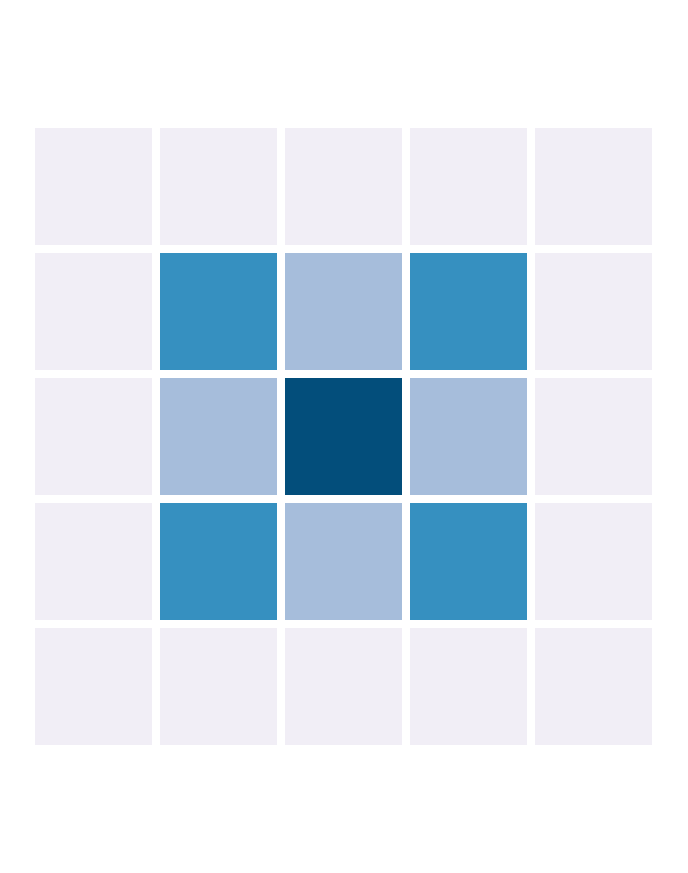
\includegraphics[width=\linewidth,trim={0.7cm 2.2cm 0.7cm 2.2cm},clip]{body/figures/63-nb_d.pdf}
       %\caption{zweite Nachbarn}
    \end{minipage}
    \hfill
    %\hspace{.1\linewidth}% Abstand zwischen Bilder
    \begin{minipage}[b]{.22\linewidth}
        %\centering
       \includegraphics[width=\linewidth,trim={0.7cm 2.2cm 0.7cm 2.2cm},clip]{body/figures/64-nb_zd.pdf}
       %\caption{zweite Nachbarn}
    \end{minipage}
    \caption[Nachbarschaftssysteme]{Nachbarschaftssystem auf regulärem Gitter. V.l.n.r.: Erste, zweite, 
    diagonale, zweite und diagonale Nachbarn}
    \label{fig_neighbours}
 \end{figure}


In Abbildung \ref{fig_neighbours} sind verschiedene Nachbarschaftssysteme für ein reguläres 
(Raster?)Gitter (exemplarisch) bezüglich 
gemeinsamer Grenzen (entspricht Manhattan-Distanz?) dargestellt. In Abbildung \ref{fig_neighbours_bl} die Anwendung auf ein 
irreguläres Gitter der Gebiete deutscher Bundesländer mit $s_i=\text{Thüringen}$.

\begin{figure} %[htb] %h=here, t=top, b=bottom, p=page of float
    \centering %Bilder mittig statt am linken Rand ausgerichtet
    \begin{minipage}[b]{.3\linewidth} % [b] => Ausrichtung an \caption --> c (=Center) t (=Top) und b (=Bottom)
        % \linewidth entspricht hier \textwidth (=Breite Textbereich)
        %\centering
        %                                 trim = links unten rechts oben
        \includegraphics[width=\linewidth,trim={1cm 1cm 1cm 1cm},clip]{body/figures/71-BL_nb_e.pdf} % [scale=0.5] oder [width=\linewidth]
       %\includegraphics[scale=0.4,trim={1cm 2cm 1cm 2cm},clip]{body/figures/popdens2018.pdf} % [scale=0.5] oder [width=\linewidth]
       %[width=\textwidth] entspricht [width=\linewidth] (=Breite einer Minipage)
       %\caption{erste Nachbarn}
    \end{minipage} % <- sonst wird hier ein Leerzeichen eingefügt
    \hfill
    %\hspace{.1\linewidth}% Abstand zwischen Bilder
    \begin{minipage}[b]{.3\linewidth}
        %\centering
       \includegraphics[width=\linewidth,trim={1cm 1cm 1cm 1cm},clip]{body/figures/71-BL_nb_e.pdf}
       %\caption{zweite Nachbarn}
    \end{minipage}
    \hfill
    %\hspace{.1\linewidth}% Abstand zwischen Bilder
    \begin{minipage}[b]{.3\linewidth}
        %\centering
       \includegraphics[width=\linewidth,trim={1cm 1cm 1cm 1cm},clip]{body/figures/73-BL_nb_zd.pdf}
       %\caption{zweite Nachbarn}
    \end{minipage}
    \caption[Nachbarschaftssysteme]{Nachbarschaftssystem auf irregulärem Gitter am Bsp der Bundesländer. 
    V.l.n.r.: Erste, zweite, diagonale}
    \label{fig_neighbours_bl}
 \end{figure}

Nachbarschaftsmatrix W wird entsprechend Kapitel 4.XX konstruiert und speichert im folgenden alle Nachbarschaftsinformationen. 
Die Einträge $w_{ij}$ entsprechen den Gewichten. Dabei werden Diagonaleinträge $w_{ii}$ auf Null gesetzt. 
In einer Standardisierung werden die Einträge der Zeile $i$ durch Zeilensumme $\sum_{j=1}^{n} w_{ij}$ geteilt.

Analog zur Erweiterung des Nachbarschaftssystems/graphen kann die Nachbarschaftsmatrix W1, W2 usw. 
mit Nachbarschaftsrelationen ersten bzw zweiten Grades gebildet werden.

\chapter{Räumliche Autokorrelation}
\label{ch:autocorrelation}

Räumliche: Autokorrelation/Abhängigkeit/Dependenz/Gebundenheit/Assoziation?/Verbindung/Zusammenhang/Zuordnung/Verbund
/Verknüpfung/Verschränkung?/Verkettung? \\

Lokation/Position/Messstelle\\

Zone/Region/Areal/Bereich\\

Gebiet/Beobachtungsraum/-gebiet

\section{Theorie und Indizes räumlicher Autokorrelation}

Ein wichtiges Konzept der räumlichen Statistik ist die \emph{räumliche Abhängigkeit} und daraus 
resultierende \emph{räumliche Autokorrelation} (engl. spatial dependence and autocorrelation).
Diese kann zum einen als Störfaktor gesehen werden, da statistische Tests verkompliziert werden. 
Bei räumlicher Autokorrelation liegt eine Abhängigkeit der Störgrößen des ökonometrischen Modells von regionalen 
Untersuchungseinheiten vor. Dies führt bei Kleinste-Quadrate-Schätzungen zu Verzerrungen der Regressionskoeffizienten 
oder Ungültigkeit der Signifikanztests. Zum anderen liefert diese zusätzliche Information Möglichkeiten 
zur räumlichen Interpolation. Während Trendprognosen eine zeitliche Autokorrelation benötigen, 
ermöglicht räumliche Autokorrelation (bzw. räumliche Persistenz) eine distanzabhängige Interpolation. 
In diesem Kapitel werden Eigenschaften und Berechnung der Statistiken untersucht.

\subsection{Einführung}

Die Korrelation (engl. correlation) beschreibt die funktionalen Beziehungen zwischen zwei 
Variablen und liefert ein Maß für den Stärkegrad der Abhängigkeit zwischen den Variablenpaaren. 
Der \emph{Bravais-Pearson'sche Korrelationskoeffizient} (auch: Produkt-Moment-Korrelationskoeffizient, Pearsons r) 
erfasst den linearen Zusammenhang zweier annähernd normalverteilter Variablen und ist zur Messung der Abhängigkeit 
metrischer und dichotomer Daten geeignet. Ein Wert von 0 gibt vollkommene Unkorreliertheit an, währen -1 exakt 
negative und +1 exakt positive lineare Korrelation bedeutet. Im Gegensatz dazu sind \emph{Spearman's rho} und 
\emph{Kendalls tau} als nichtparametrische/parameterfreie Rangkorrelationskoeffizienten auf ordinalskalierten Daten 
ohne Verteilungsannahmen anwendbar.

Autokorrelation misst die Korrelation eines Merkmals mit sich selbst und wird zwischen (zeitlich oder räumlich) 
benachbarten Beobachtungen erfasst. Bei Messungen (bezüglich) eines Beobachtungsobjektes im Zeitverlauf ist es (i.A.) 
wahrscheinlich, dass zeitlich nahe beieinander liegende Beobachtungen ähnlichere Messwerte liefern als solche mit 
größerem zeitlichen Abstand. Messwerte ändern sich graduell(stetig) im Zeitverlauf, wenn auch nicht streng monoton. 
Zeitliche Autokorrelation misst in der Zeitreihenanalyse den Grad der Assoziation zwischen Beobachtungsfolgen 
(bzw. Signalen) oder Folgen von Zufallsvariablen in Einheiten bestimmter, meist äquidistanter, als Lags bezeichnete 
Zeitabstände. Eine Folge wird zeitlich verschoben und zu sich selbst in Beziehung gesetzt. 
Die Anwendung auf zwei verschiedene Folgen/Signale wird hingegen als Kreuzkorrelation bezeichnet. 
Auf diese Art wird allgemeine/lineare?, nicht-zufällige/signifikante Beziehung zwischen zeitlich versetzten 
Folgengliedern gesucht. Ergebnisse werden in der \emph{Autokorrelationsfunktion} ($\mathbf{ACF}$) zusammengefasst.

\textbf{FischerGetis2009 p.260}\\

Analog zu diesen bekannten Einführungsbeispielen existieren Koeffizienten (bzw. Indizes) zur Erfassung einer 
Autokorrelation von räumlich verteilten Messungen. In der räumlichen Analyse liegt ebenfalls die Annahme zugrunde, 
dass Beobachtungswerte ähnlicher sind, je näher beieinander ihre Positionen im Raum liegen.
(dass räumlich benachbarte Beobachtungen einer Variablen/Attributs ähnlicher sind als weit entfernte). 
Dieses Konzept wird durch \emph{Toblers erstes Gesetz der Geographie} aus Abschnitt \ref{subsec:tobler} begründet. 
Dieser Zusammenhang ist bekannt als positive räumliche Autokorrelation, also eine Korrelation der Variablen mit sich selbst. 
Es werden zwei Informationen verknüpft: die Ähnlichkeit der Beobachtungen/Messwerte mit der Ähnlichkeit der Positionen. 

%ERGÄNZUNGEN

Daten aus Punktprozessen und Geostatistik lassen sich direkt über die euklidische Norm räumlich in Beziehung setzen. 
Für Gitterdaten liegen jedoch diskrete? Raumvariablen vor, und die räumliche Anordnung der Daten wird anders codiert/konstruiert/beschrieben.

Die folgende Konzepte sind insbesondere für Gitterdaten (engl. lattice data) relevant, wie im Abschnitt 4.3 definiert. 
Im Gitter können sowohl Zonen als auch Punkte angeordnet werden. Die räumliche Information liegt hier diskret z. B. in Form 
einer Regionenvariable $s$ vor. Dieses (Daten)Gitter muss um Nachbarschaftsinformation (in Form einer Matrix?) ergänzt werden, 
um für das weitere Vorgehen/Anwendung die Nachbarschaftsrelation (paarweise) eindeutig zu definieren. 
Nachbarschaften können auf unterschiedliche/zahlreiche Arten konstruiert werden. 

\section{Indizes und Tests der Autokorrelationsmessung}
Räumliche Autokorrelation vergleicht parweise die Ähnlichkeit von Merkmalswerten 
$z_i=Z\left(s_i\right)$ mit $z_j=Z\left(s_j\right)$ 
in Bezug zur Nähe ihrer Lokationen (Raumpunkte/Polygone etc.) $s_i$ und $s_j$ und leitet die tendenzielle 
(funktionale?) Beziehung ab. 
Häufig verwendete Maße globaler Autokorrelation sind Moran’s I und Geary’s C, welche Spezialisierungen des folgenden 
Kreuzproduktes darstellen (siehe Getis 1991 p.  ) (vgl. Anselin 1995):

Ausgehend von der grundlegenden Repräsentation einer räumlichen Statistik als Kreuzprodukt 
\begin{equation}
    \Gamma_{ij} =\sum_{i=1}^n \sum_{j=1}^n W_{ij} Y_{ij}
\end{equation}
(mit $\Gamma$ als Maß räumlicher Autokorrelation von $n$ georeferenzierten Beobachtungen) werden weitere Statistiken entwickelt. 
Dabei repräsentieren die Gewichte $w_{ij}$ der Nachbarschaftsmatrix $W$ die räumliche Beziehung einer 
jeden Lokation $i$ zu allen anderen Standorten $j$. 
In Variablenmatrix $Y$ werden die metrischen?/stetigen(continuous) Realisierungen $y_j=Y\left( s_j \right) $
an verschiedenen Positionen $s_j$ um $s_i$ herum in Beziehung gesetzt. 
Die Werte interagieren wahlweise paarweise additiv $\left(y_i+y_j\right)$, multiplikativ $\left(y_i \cdot y_j\right)$, 
differenziert $\left(y_i-y_j\right)$ oder dividiert $\left(y_i / y_j\right)$. (Fischer Getis 2010, S. 259)
Eine wichtige Voraussetzung ist ein räumlich konstanter Mittelwert $ \bbbe\left[Y\left(s\right)\right]=\mu$ ,
welcher wie genau.....??(Schabenberger,Gotway 2005, p.21). 
Ähnlichkeit der Attributswerte $y_i$ und $y_j$ kann durch folgende Maße ausgedrückt werden:
\begin{eqnarray}
    U_{ij} & = &\left (y_i - \mu \right) \left( y_j-\mu \right) \\
    U_{ij} & = &\left( y_i-\bar{y} \right) \left( y_j-\bar{y} \right) \\
    U_{ij} & = &\left| y_i-y_j \right| \\
    U_{ij} & = &\left( y_i-y_j \right)^2 \\
\end{eqnarray}
Praktisch relevante Beispiele sind aufgrund guter Berechenbarkeit und Interpretierbarkeit 
das Kreuzprodukt der Form $\operatorname{REF1}=\left( y_i-\bar{y} \right) \left( y_j-\bar{y} \right)$ für Morans Index 
sowie quadrierte Differenzen $\operatorname{REF2}=\left( y_i-y_j \right)^2$ für Gearys c. 
Ist $\bar{y}$ konsistent für $\mu$, dann ist auch $\bbbe\left[ \left(y_i-\bar{y}\right)\left(y_j-\bar{y}\right) \right]$ 
konsistenter Schätzer von $\operatorname{Cov} \left( y_i , y_j \right)$. (BEWEIS?)
Somit gibt $Y$ eine (spezifische) Beziehung zwischen Realisierungen/Beobachtungeswerten an Punkt $i$ 
zu allen anderen Orten $j$ der nichträumlichen Variablen wieder. 
Weisen $W$ und $Y$ ähnliche Struktur auf (d.h. sowohl hohe als auch niedrige Werte liegen in in den 
gleichen $\left(i,j\right)$-Zellen), so liegt ein hoher Grad positiver räumlicher Autokorrelation vor. 
Bei gegenläufig übereinstimmenden Werten in den gleichen $(i,j)$-Zellen) liefert $\Gamma$ negative Autokorrelation. 
Für eine sinnvolle Bewertung muss $Y$ den räumlichen Bezug widergeben und $W$ die räumliche Struktur sinnvoll repräsentieren. 
Weist auch nur eine der beiden Matrizen eine zufällige Verteilung auf, so liefert $\Gamma$ ein Maß von Null.

Zahlreiche Maße und Tests sind auf dieser Basis etabliert und unterscheiden sich voneinander in der Struktur der Matrizen $W$ und $Y$. 
Es können globale sowie lokale Maße und Tests abgeleitet werden. 
Globale Statistiken aggregieren die Autokorrelation über die Gesamtheit der Daten. 
Alle Elemente der $W$ und $Y$ Matrix mit ihren räumlichen Assoziationen werden gemeinsam ausgewertet und resultieren in einem einzelnen Ausgabewert.
Lokale Maße (engl. Local indicators of spatial association – LISA) bewerten Autokorrelation üblicherweise mit Fokus auf einzelne räumliche Einheiten/Gebiete. 
Somit beeinflusst nur eine Reihe der $W$ und $Y$ Matrix die Berechnung direkt. [FischerGetis2009 pp 26X-262]
Sie geben für die Nachbarschaftswerte um eine feste/bestimmte Position den Grad der Abweichung von einer zufälligen Verteilung an. (Anselin et al. 2000) 
Sie erlauben die Zerlegung globaler Indikatoren (wie Morans I) in die Anteile, welche die Messwerte einzelner Lokationen beitragen. (Anselin 1995, S. 94)

In der Geostatistik drückt das Semi-Variogram den Grad der räumlichen Autokorrelation in einem Datensatz aus. 
Analog hierzu wird eine Statistik als distanzabhängige Funktion betrachtet, indem ihre I-Werte für verschiedene Distanzbänder auf Basis der 
Nachbarschaftsmatritzen $W(1), W(2),\ldots,W(q)$ für Nachbar ersten bis q-ten Grades abgetragen werden.

\subsection{Globale Autokorrelationsmaße}

\subsubsection{Gamma}
Als Basisfunktion aller weiteren Maße und Tests wurde diese Statistik (3.1) vorgestellt. 
Durch die Randomisierung der Werte der Y Matrix in einer Reihe von Simulationsläufen wird (die Hülle einer) eine Referenzverteilung erzeugt. 
Der tatsächliche Wert liegt im Signifikanzbereich

\subsubsection{Join-count}
Darüber hinaus existiert der joint-count Index für nominal klassifiezierte Daten...

\subsubsection{globaler Moran Index}
Der globale Moran Index (engl. global Moran’s I) 
misst als Statistik den Grad sowohl positiver als auch negativer Autokorrelation. 
Er ist als Produktmoment wie der Pearson Korrelationskoeffizient strukturiert. 
Jedoch wird, unter zusätzlichen Integration der räumlichen Information aus Matrix $W$, 
die Autokorrelation einer Variablen mit sich selbst gemessen statt einer klassischen Korrelation zweier Variablen miteinander. 


\begin{definition}[Moranscher Index] \label{def:global-moran}
    Analog zur Pearson Statistik erfolgt eine Skalierung. 
    Der Vorfaktor  $n \big/ \left( \sum_{i=1}^{n} \sum_{j=1}^{n} w_{ij} \sum_{i=1}^{n} \left(y_i-\bar{y}\right)^2 \right) $ 
    ergibt die folgende Statistik zur Beziehung eines Datenpunktes (e.g. Einkommen) mit seinen Umgebungswerten (Moran 1950, p.22):
    
\begin{equation}
    I=\frac{n}{\sum_{i=1}^{n}\sum_{j=1}^{n} w_{ij}} 
        \frac{\sum_{i=1}^{n}\sum_{j=1}^{n}{w_{ij} \left( y_i-\bar{y} \right) \left( y_j-\bar{y} \right) }}  
        {\sum_{i=1}^{n} \left( y_i-\bar{y} \right)^2} ~ , ~ i \neq j
\end{equation}

Hierbei sind: 
	$y_i=$ i-ter Beobachtungswert der räumlichen Variable $y$
	$w_{ij}=$ Distanzgewichte der räumlichen Beobachtungen(?)
	$n=$ Anzahl Beobachtungen/Stichprobengröße
	$S_0= \sum_{i=1}^{n} \sum_{j=1}^{n} w_{ij}$

\end{definition}

Matrix $W$ kann in beliebiger Form aufgestellt werden und beschränkt die räumliche Interpretation nicht. 
Somit ist der Test sehr flexibel, aber auch auch anfällig gegen Ausreißer und Fehlspezifikationen der Nachbarschaftsbeziehungen. 
Matrix $Y$ in Form einer Kovarianzmatrix misst die Abweichungen der Beobachtungen vom Mittel aller Beobachtungen.
(Fischer, Getis 2010, S 263-265)
Es ist Konvention, keine Selbstassoziation zu erfassen (i ist ungleich j). 
Durch Standardisierung der Gewichte können Ausgabewerte der I-Statistik auf die Spanne [-1,1] eingeschränkt werden. 
Die lokale Variante als Weiterentwicklung der Moran I Statistik wird in Abschnit XXX behandelt.
(?)Die Nullhypothese geht davon aus, dass keine  ......

schernthanner S. 49
Dpl Arbeit Strauß S.18
Fischer Getis 2010 S. 265
Haining S. 243
Goodchild S. 16

\subsubsection{Gearyscher Index}

Bekannt als Gearysches Nachbarschaftsverhältnis oder Gearyscher Index (engl. Geary’s c, Geary's Contiguity Ratio), 
liegt der Unterschied zur Moran Statistik in der Berechnung der Attribute durch Kreuzprodukt als $Y_{ij}=\left(y_i-y_j\right)^2$. 
Die Gewichtsmatrix X kann wie im Moran Index verwendet werden und erlaubt die gleiche Flexibilität. Geary's c ist jedoch sensitiver bezüglich lokaler Autokorrelation.

\begin{equation}
    c=\frac{n-1} {2 \sum_{i=1}^{n} \sum_{j=1}^{n} w_{ij}} 
        \frac{\sum_{i=1}^{n}\sum_{j=1}^{n} {w_{ij} \left(y_i-y_j\right)^2}} 
        {\sum_{i=1}^{n}\left(y_i-\bar{y}\right)^2} ~, ~ i\neq j
\end{equation}

Die Ausgabewerte liegen im Bereich [0,2]. Ein Wert von 1 impliziert, dass keine räumliche Autokorrleation vorliegt.
FischerGetis2009 p.265

\subsubsection{Statistische Inferenz und Tests}

Analog zur allgemeinen Mantel Statistik ist Inferenz für die I und c Statistik auf Basis von Permutationstests, 
Monte-Carlo Tests oder auf asymptotischen Verteilungen von I und c basierten Approximationstests möglich. 
Um Erwartungswert und Varianz von I und c abzuleiten sind zwei grundlegende Annahmen(Voraussetzungen) über die 
zufällige Veteilung der Y-Werte möglich. 
Die erste Annahme einer Normalverteilung (engl. Gaussianity assumption) sieht jeden einzelnen Y-Wert $y_i$ 
als Realisierung einer eigenen gaussschen Zufallsvariablen mit Mittel $\mu$ und Varianz $\sigma^2$, 
wobei jede Raumeinheit eine eigene Normalverteilung aufweist (wirklich?). 

In der zweiten Annahme (engl. randomness assumption) werden Mittel und Varianz abgeleitet unter der Annahme 
einer randomisierten Zuordnung/zufälligen Positionierung (engl. randomizing) der Y-Werte $y_i$ zu den einzelnen Gitterlokationen.
Diese Zufallsverteilungsannahme interpretiert die Y-Werte als Realisierungen einer unform gleichverteilten Zufallsvariablen 
(d.h. alle Realisierungen gleich wahrscheinlich...wirklich?) [Fischer,Getis 2009 p.264].

Die Randomisierungsannahme führt gegenüber der einfacheren Normalverteilungsannahme einen zusätzlichen Korrekturterm der Kurtosis ein. 
Entspricht die Kurtosis der Attributswertverteilung der einer Normalverteilung, dann stimmen die Testergebnisse unter beiden Annahmen überein. 
Um so mehr die Verteilung von einer Normalverteilung abweicht, desto kompensiert die Randomisierungsannahme durch Anheben der Varianz 
und abnehmende Standard deviate? [Bivand 2013, p.280]

Beide Annahmen (\glqq Gaussianity \grqq{} und \glqq randomness \grqq{}) resultieren im gleichen Erwartungswert der Indizes,
\begin{eqnarray}
    \bbbe_{g} \left[I \right]=\bbbe_{r}\left[ I \right]=\frac{-1}{(n-1}
    \bbbe_{g} \left[c \right]=\bbbe_{r}\left[ c \right]=1
\end{eqnarray}

während die Varianzen je nach Annahme voneinander abweichen:
(weitere Details: Cliff and Ord 1981, p.21)

Ein Hauptgrund für die Popularität der Statistiken ist die asymptotische Normalverteilung der Ausgabewerte mit zunehmendem $n$ (Cliff and Ord 1973). 
Der Index kann hiermit durch z-Werte der Normalverteilung bewertet werden. 
Als Korrelationsindex ist der Moran I-Wert eine dimensionslose Größe. 
Die Ausgabewerte sind nicht direkt interpretierbar, sondern erst im Bezug zu Verteilungsmomenten. 
Gilt $I>\bbbe\left[I\right]$, dann weisen räumlich verbunde Lokationen tendenziell ähnliche Attributswerte auf. 
Der Stärkegrad dieser positiven Autokorellation steigt mit dem Abstand $\left| I-\bbbe\left[ I \right] \right|$ an. 
Für $I<\bbbe\left[ I \right]$ hingegen weisen räumlich verbundene Lokationen tendenziell unterschiedliche Attributswerte auf. 
Die Interpretation der c Statistik von Geary verhält sich genau umgekehrt. 
Für Werte $c>\bbbe\left[c\right]$ liefern räumlich benachbarte Positionen tendenziell unterschiedliche Werte 
und vice versa für $c<\bbbe\left[c\right]$. [Schabenberger Gotway 2005, p.22]

Um die Signifikanz der Abweichung vom Erwartungswert zu bewerten, wird der Ausgabewert standardisiert, 
indem der Erwartungswert abgezogen und diese Differenz durch die Wurzel der Varianz (in Abhängigkeit der räumlichen Gewichte) geteilt wird. 
\begin{equation*}
    Z = \frac{I- \bbbe \left[ I \right] } {\sqrt{Var{I}}}
\end{equation*}

Dieses Standardmaß liefert im Vergleich zur Normalverteilung eine Wahrscheinlichkeit für das Auftreten des beobachteten Statistik-Wertes unter der Nullhypothese, 
dass keine räumliche Abhängigkeit bezüglich der gewählten räumlichen Gewichte vorliegt. 
Zumeist ist dieser Test einseitig gerichtet, mit der Alternativhypothese, dass der realisierte Statistikwert signifikant größer als ihr 
Erwartungswert ist (keine signifikant kleinere Realisierung erfasst). 
Eine Ablehnung der Nullhypothese (H0:räumlich zufällige Verteilung) impliziert mit entsprechendem, (zuvor fixierten!) Niveau (e.g. 95 \% ) Sicherheit 
dass räumliche Autokorrelation exisitiert. [Bivand 2013, p. 278]

Voraussetzung für die korrekte Signifikanz im Einsatz als Test ist es, dass im Mittel kein systematisches Muster/Struktur(irung)/Formation? vorhanden ist. 
Getestet werden ausschließlich angepasste Trend-Modelle (engl. (centring) mean model) mit konstantem (konstant worüber?) Mittel. 
Verbleibende Muster/Autokorrelation nach der Mittelung ist auf räumliche Beziehung innerhalb der Gewichtsmatrix zurückzuführen. 

In numerischen Testversuchen/läufen werden räumlich unkorrelierte Zufallswerte für jedes Gebiet/Punkt konstruiert. 
Durch Plotten solcher „Rauschkarten“ ließe sich auch optisch kein Muster ausmachen. 
Wird in diese Daten ein einfacher linearer Trend eingeführt, etwa durch leichte Zunahme in West-Ost Richtung, 
so darf aus den Testwerten dieses Modells keine Autokorrelation abgeleitet werden. 
Im Westen lokalisierte Werte liegen trendbedingt im Durchschnitt unter dem globalen Mittelwert und im Osten gelegene Werte darüber. 
Es liegt jedoch hierdurch nur eine globale,lineare Verschiebung des ursprünglichen „Rauschbildes“ vor, 
welches für lokale Nachbarschaftsbeziehungen weiterhin keinerlei Muster (bzw. Autokorrelation) erkennen ließe. 
Trotzdem würden die globalen c und I Statistiken auf derartige globale Trends ansprechen/reagieren und signifikante Autokorrelation suggerieren, 
da sie ursprünglich für homogene Mittelwerte und Varianzen ausgelegt sind. 
Eine derartige Fehlspezifikation des Modells kommt in der Fachliteratur durchaus vor [McMillen2003]. 
Eine Beispielrechnung liefern [Schabenberger, Gotway 2005, pp.22-23]

Da eine Annahme der Stationarität des Erwartungswert insbesondere über große Beobachtungsgebiete oft nicht sinnvoll ist, werden zwei Auswege verfolgt.
\begin{enumerate}
    \item Ein systematischer (linearer) Trend wird durch Kovariablen eines linearen, mittelnden Modells (engl. mean model) erfasst und korrekt gewichtet/spezifiziert, 
    bevor ein Test der Residuen (Erwartungswert gleich Null) gültige Aussagen liefert. [Bivand S. 277] 
    Für das Modell $Y(s)=X(s)\beta+e$ werden Fehlerquadrate minimiert (engl. ordinary least squares - OLS) um $\beta$ zu schätzen. 
    Die Kontrolle erfolgt mittels Moran oder Geary Statistik über die Residuen $\hat{e}_i=y_i-x\prime(s_i) \hat{\beta}$. 
    Weitere Details im Kapitel...? [Schabenberger, Gotway 2005, p. 23]
    \item  Selbst unter global heterogenem Erwartungswert kann es sinnvoll sein, von konstanten Erwartungswerten auszugehen. 
    Unter dieser Annahme wird die Berechnung der Autokorrelation lokalisiert. 
    Dieser LISA-Ansatz lokalisierter Indikatoren wird im folgenden Abschnitt XXX eingeführt.
\end{enumerate}

Der Standard Morantest unter der Normalverteilugnsannahme entspricht dem Morantest der Regressionsresiduen eines Modells, welches lediglich mit einem Intercept ausgestattet wird. 
Dies zeigt, dass zusätzliche Kovariablen eingeführt werden können (over and above the intercept?), um Missspezifikationen auszubügeln. 
Mit der gleichen Konstruktion kann zudem eine Sattelpunkt-Appriximation statt der analytischen Normalverteilungsannahme (Tiefelsdorf 2002) 
sowie exakter Tests (Tiefelsdorf, Hepple, Bivand) verwendet werden. 
Diese Methoden sind jedoch numerisch aufwendig, für moderate Datensätze wie im vorliegenden Fall jedoch noch praktikabel. 
Wie die Anwendung in Kapitel 4 zeigt, sind die Unterschiede für globale Tests gering, insbesondere falls Anzahl an Lokationen nicht klein ist. 
Für lokale Maße sind die Unterschiede zwischen Normalverteilungsannahme und Sattelpunktapproximation und exaktem test hingegen ausgeprägter [Bivand 280].

Aufgrund der Sensitivität dieser Tests bezüglich der Grundannahmen und Konstruktion der Nachbarschaftsbeziehungen wird oft auf Simulationen (als Ergänzung?) zurückgegriffen.

\subsubsection{Monte-Carlo Simulation}

In der Monte-Carlo Simulation oder bootstrap permutationsbasierten Tests werden die realisierte Attributswerte neu auf die Lokationen/räumlichen Einheiten verteilt, 
randomisiert in vielen Zufallsläufen. 
Im Gegensatz zur Simulation lokaler Statistiken (Referenz) liegen genug Beobachtungen für eine sehr große Anzahl Permutationen 
zur ausreichenden Wiederholung der Simulation ohne Gefahr von Wiederholungen vor. 
Somit werden Inferenzfehler vermieden/minimiert?. 
Jedoch beseitigen sie nicht die Abhängigkeit der globalen Statistik von Autokorrelationen aller möglichen Quellen 
und liefern keine Hinweise/Anhaltspunkte zum Enstehungsprozess der Daten. 
Die Simulationsanwendung darf nicht von Situationen ablenken, in denen bessere Modellanpassungen 
oder genauere Spezifikationen der untersuchten Variablen nötig sind. [Bivand 2013, p. 278]
Die praktische Anwendung auf die reale Datengrundlage in Kapitel 6.XX liefert weitere Details zur Berechnung und Interpretation.

\subsubsection{Variogram}

Räumliche Korellogramme (engl. Spatial Correlograms) bzw. Variogramme(?) dienen

\subsubsection{G-Statistik}
Getis, Ord - G-Statistic
AnselinRey2010 Chapter 10

\subsubsection{H-Statistik}

\subsection{Lokale Autokorrelationsmaße}

Globale Autokorrelationsmaße aggregieren über die einzelnen lokalen Nachbarschaftsbeziehungen der räumlichen Einheiten. 
Die Statistik für Matrizen(verknüpfung?) $M_2$ von Mantel aus Abschnitt XX kann als Summe der einzelnen Beiträge $m_i$ aller Datenpunkte $s_i$ geschrieben werden.
\begin{equation}
    M_2 = \sum_{i=1}^{n}\sum_{j=1}^{n}{w_{ij} u_{ij}} = \sum_{i=1}^{n} m_i ~ , ~ i\neq j? \text{und} m_i = \sum_{j=1}^{n} {w_{ij} u_{ij}}
\end{equation}

Die Beiträge $m_i$ werden hierbei als lokales Autokorrelationsmaß der Lokation $s_i$ interpretiert. 
In gleicher Weise lassen sich Spezialisierungen von $M_2$ wie Black-White join count, die Moran I sowie Geary c Statistik in ihre lokalen Einzelbestandteile zerlegen 
und lokale Tests konstruieren [Schabenberger, Gotway 2005, p. 23]. 

Mit ihrer Hilfe sollen zum einen räumliche Anhäufungen und Zusammenballungen (engl. Cluster), also Beobachtungen mit sehr ähnlichen Nachbarn (bezüglich des Attributs) ermittelt werden. 
Zum anderen werden lokale Hochburgen bzw. stationäre Schwerpunkte mit außergewöhnlichen Spitzenwerten / kritische Risiko-bzw. Gefahrenherd (engl. Hotspots), 
das heißt Beobachtungen mit sehr unterschiedlichen Nachbarn, erfasst /sondiert werden.


\chapter{Räumliche Regression}

Regressionsmodelle stellen die primäre Klasse zur räumlichen Modellanalyse dar. 
Der Unterschied in der räumlichen Struktur zwischen stetigen Punktlokationen der Geostatistik und 
diskreten Gebietsdaten/Raumeinheiten der Raumanalyse(?)als Partition des Gesamtraumes spiegelt sich auch in den Regressionsmodellen wieder. 
Der Georegression liegt die Stationarität der Kovarianz im Raum als fundamentale Anahme zugrunde. 
Die Verteilungsmodellierung der Residuen erfolgt mittels Variogram und zugehörigen Kovariogrammen.
Im Gegensatz dazu wird im folgenden die Annahme der Stationarität ersetzt durch 
räumlich autoregressive Annahmen auf Grundlage der Gewichtsmatrix. 
% Deren spezifische Details umfasst zum einen die Konstruktion der Regressionsresiduen 
% im räumlich bezogenen Fehlermodell (spatial error model).
% Zum anderen die verzogenen Regressoren(?) im räumlich verzogenen Modell (spatial lag model)
% [SEM und SLM zu spezifisch hier, besser SAR und CAR unterscheiden]

Peter Whittle forschte ab 1949 an der Zeitreihenanalyse und übernahm eine analoge 
Theorie für stationäre Gaußprozesse auf räumliche Prozesse (Whittle 1954). Gani S.187 enthält eine 
persönliche Zusammenfassung aus Whittles Sicht und seiner Zusammenarbeit mit Matern, Bartlett und weiteren bekannten
Namen des Gebietes der Stochastik. 

\section{Spatial Statistics – Allgemeine Räumliche Autoregression}

Im folgenden werden räumliche (Auto-)regressionsmodelle (engl. spatial autoregressive models) eingeführt. 
Wie in Kapitel XX erläutert, ist die Annahme unabhängig identisch verteilter Beobachtung aufgrund 
(inhärenter/impliziter) räumlicher Abhängigkeiten nicht zweckmäßig/gerechtfertigt (heteroscedacticity?). 
Zudem muss der Einfluss räumlicher Autokorrelation getrennt werden von den (impliziten/inhärenten?) 
räumlichen/lokalen Unterschieden der (räumlichen/multivariaten) Verteilung.

Im folgenden wird die relevante Menge der Raumeinheiten $\left\{ R_1,\ldots,R_n \right\}$ durch ihre 
Indizes $i=1,\ldots,n$ vereinfacht repräsentiert. Insbesondere wird es sich immer um 
die Stichprobeneinheiten handeln. Eine uamfassendere Grundgesamtheit ist nicht gegeben [?].
Als lineares Grundmodell für Abhängigkeiten zwischen einzelnen Einheiten dient

\begin{equation} \label{eq-6.1:reg-mod-gen}
    Y_{i}=\beta_{0}+\sum_{j=1}^{k} \beta_{j} x_{ij} +e_{i} \, , \, i=1,\ldots,n
\end{equation}
mit $Y_i$ als relevantes Attribut für jede Raumeinheit $i$ und $(x_{ij}:j=1,\ldots ,k)$ als Menge der
Erklärungsattribute von $i$ welche den Wert $Y_{i}$ beeinflussen. Der Hauptunterschied zur Georegression ist
die Modelierung von $e_{i}$ über ein eigenes explizites lineares Model statt als zufälligen Fehlerterm $\varepsilon_{i}$.

Korrelierte Beobachtungen werden in Matrixschreibweise über Zusammenhang \eqref{eq-6.2:reg-mod} modelliert.

\begin{equation} \label{eq-6.2:reg-mod}
    \mathds{Y} = \mathds{X}^{\intercal} \beta + \nu 
\end{equation}
%\mathds{1}
%\bbbe
%\mathbb{I}

Die Störgröße $\nu$ wird als multinomial verteilter Zufallsvektor aus standardnormalverteilten(?) Fehlertermen 
mit $\bbbe[\nu]=0$ angenommen, sodass
\begin{equation*}
    \bbbe[Y]=\mathds{X} \beta
\end{equation*}
gilt.
Während die Störterme $\nu$ im klassischen Regressionsmodell als i.i.d angenommen werden, benötigen wir nunmehr 
eine Möglichkeit, räumlich auftretende Korrelationsstrukturen in dieses Modell zu integrieren. Zum einen 
lässt sich der Fehlerprozess als \emph{raumstrukturell autoregressiver Prozess} 
(engl. spatially autoregressive process - SAR)
\begin{equation*}
    \nu = \rho W \nu + \varepsilon
\end{equation*}
erfassen. Zum anderen ist eine Integration als \emph{raumstruktureller Gleitmittelprozess} (engl. spatially 
moving average process - SMA)
\begin{equation*}
    \nu = \rho W \varepsilon + \varepsilon
\end{equation*}
denkbar mit Gewichtsmatrix $W$, Autoregressionsparameter $\rho$ und $\varepsilon$ als 
Vektor von i.i.d.-verteilten Störgrößen. 


Die Struktur der Korrelation zwischen Gebieten wird durch eine bestimmte(?) Varianzmatrix $V$ erfasst.
Der (lineare) Trend $Y = X^{T} \beta$ wird in linearer 
Abhängigkeit von (unabhängiger, exogener) Erklärungsvariable $X$ bzw. mehreren 
Kovariablen (engl. covariate, control variable) $X_1,\ldots,X_k$ modelliert.  

Liegt als Output keine (multivariate) Normalverteilung vor, kann eine Transformation der 
abhängigen Reaktionsvariable bzw. Zielgröße (Regressand) helfen. 

Es folgen verschiedene Ansätze von Korrelationsstrukturen, verwirklicht in den Modellklassen 
der Simultaneous Autoregressive Models (SAR) und Conditionally Autoregressive Models (CAR) sowie....

\section{Simultaneous Autoregressive Models - SAR}

Das Hauptziel ist die Modellierung der Kovarianzstruktur von $\nu$ unter Berücksichtigung der 
räumlichen Abhängigkeiten zwischen den Instanzen.
Die räumliche Gewichtsmatrix $W=[w_{ij}:i,j=1,\ldots,n]$ 
erfasst die diskrete Raumstruktur und räpresentiert oft ein Maß räumlicher Nähe. Größere Werte $w_{ij}$ 
bedeuten hierbei größere Nähe und Einfluss von $i$ und $j$ aufeinander. Jedes Residuum $e_{i}$ wird 
durch die Residuen der Nachbargebiete $j$ mit positiven paarweisen Raumgewichten $w_{ij}$ beeinflusst. 
Diesen Einfluss räpresentiert das lineare Teilmodell
\begin{equation} \label{eq-6.2:reg-st}
    \nu_{i}=\sum_{j=1 ; j \neq i}^{n} \alpha(w_{ij}) \nu_{j} + \varepsilon_{i}
\end{equation}   
mit $\alpha(w_{ij})$ als Einflussfunktion und $\varepsilon_{i}$ als Anteil des Residuums, welcher 
nicht durch andere Einheiten beeinflusst wird. Da die Gewichtsmatrix bereits große Flexibilität durch 
die Spezifikation der Raumstruktur bietet, wird die Funktion $\alpha$ auf die einfachste 
denkbare Form eines räumlich unabhängigen Skalierungsfaktors $\rho$ reduziert.
Folglich resultiert aus \eqref{eq-6.2:reg-st} der Zusammenhang
\begin{equation}\label{eq-6.3:reg-err}
    \nu_{i}=\rho \sum_{j = 1}^{n} w_{ij} \nu_{j} + \varepsilon_{i} \, , \quad 
    \varepsilon_{i} \sim \mathcal{N}(0,\sigma^{2}) \, , \, i= 1,\ldots,n
\end{equation}
als lineares Regressionsmodell (ohne Interzeptor) für jedes Residuum $\nu_{i}$ im Regress auf 
seine Nachbarn $\nu_{j}$ mit Koeffizienten $\rho \, w_{ij}$. Aufgrund dieser Regression der 
Residuen auf \glqq sich selbst \grqq{} wird dieses Teilmodell 
als \emph{Räumlich Autoregressives Modell der Residuen} 
(engl. spatial autoregressive model of residual dependencies) 
bezeichnet (Whittle 1954), inspiriert von den Begrifflichkeiten der Zeitreihentheorie. 
Selbstregression durch individuelle Residuen wird durch Voraussetzung $w_{ii}=0$ verhindert. Alternativ kann für die 
Summation auch $i \neq j$ vorausgesetzt werden.

Nehmen wir für die intrinsischen Restkomponenten $\varepsilon_{i}$ eine \emph{i.i.d.} Verteilung gemäß 
\begin{equation} \label{eq-6.4:err-err}
    \varepsilon_{i} \sim \mathcal{N}(0,\sigma^{2}) \, , \, i=1,\ldots,n
\end{equation}  
an, so gilt $\bbbe[\varepsilon_{r}]=0$ sowie $\bbbe[\varepsilon_{r}\varepsilon_{s}]=0$ 
und $Var(\varepsilon_{r})=\sigma_{r}^{2}$. 
Parameter $\rho$ steuert den Grad der Regression(?). 
Für $\rho = 0$ wird jedes Residuum $e_{i}$ auf seine eigene intrinsische 
Komponente $\varepsilon_{i}$ reduziert und räumliche Abhängigkeiten verschwinden ganz. 
In diesem Fall wird Modell \eqref{eq-6.2:reg-mod} zu einem einfachen linearen Regressionsmodell reduziert.
Für große $\rho$ werden die (positiven und negativen) räumlichen 
Abhängigkeiten dominanter. Daher wird $\rho$ auch als \emph{Parameter räumlicher Abhängigkeit} 
bezeichnet. 
Außerdem muss für beliebige Paare $ij$ und $kh$ mit positiven räumlichen 
Gewichten $w_{ij},w_{kh}>0$ und einem nicht verschwindenden Parameter $\rho \neq 0$, 
\begin{equation*}
    \frac{\rho \, w_{ij}}{\rho \, w_{kh}} = \frac{w_{ij}}{w_{kh}}
\end{equation*}
gelten. Somit ist die relative Stärke ihrer räumlichen Dependenz ausschließlich durch ihre Gewichte bestimmt.
Das Modell bietet somit eine natürliche Zuordnung/Unterteilung der Verantwortlichkeit, 
da $\rho$ das allgemeine Niveau räumlicher Abhängigkeit bestimmt und die räumliche 
Struktur der Gewichtsmatrix $W$ ihre relative Stärke zwischen individuellen Paaren räumlicher Einheiten.

Zusammen formen \eqref{eq-6.3:reg-err} und \eqref{eq-6.4:err-err} 
das \emph{Autoregressive Modell der Residuen} (engl. autoregressive residuals?) nach Whittle (1954)
in Matrixschreibweise, 
\begin{equation}\label{eq-6.5:reg-vec}
    \nu=\rho W \nu + \varepsilon \quad , \, \varepsilon \sim \mathcal{N}(0,\sigma^{2} \mathds{I}_{n}) \, , 
    \, \operatorname{diag}(W)=0
\end{equation}
Entwickelt wurde diese Form durch Ord (1975) ?, welcher auch vom 
räumlich autoregressiven Prozess erster Ordnung sprach.
Die Modellgleichung $\nu=\rho W \nu + \varepsilon$ lässt sich direkt nach $\varepsilon$ 
umstellen und ergibt somit $(\mathds{I}_{n} -\rho W) \nu =\varepsilon$. 
Sofern Inverse $(\mathds{I}_{n} -\rho W)^{-1}$ existiert, lässt sich die 
folgende Lösung für $\nu$ in reduzierter Form erhalten
\begin{equation} \label{eq-6.6:reg-red}
    \nu=(\mathds{I}_{n} -\rho W)^{-1} \varepsilon \, , \, 
    \varepsilon \sim \mathcal{N}(0,\sigma^{2} \mathds{I}_{n}) \, , \, \operatorname{diag}(W)=0
\end{equation}


\subsection{Räumlich fehlerbezogenes Modell - SEM}

Die Integration der autoregressiven Residuen aus \eqref{eq-6.5:reg-vec} in das ursprüngliche 
Regressionsmodell \eqref{eq-6.2:reg-mod} der Form $Y=X \beta + \nu$ liefert nun das 
Gesamtmodell 
\begin{equation} \label{eq-6.7:sem-mod}
    Y=X \beta + \nu \, , \, \nu=\rho W \nu + \varepsilon \, , \, 
    \varepsilon \sim \mathcal{N}(0,\sigma^{2} \mathds{I}_{n}) \, , \, 
    \operatorname{diag}(W)=0
\end{equation}
und wird als \emph{räumlich fehlerbezogenes Modell} 
(engl. spatial error model - SEM) mit räumlich autokorrelierten Fehlertermen/Störungen bzw. 
raumstruktureller Autokorrelation im Fehlerterm bezeichnet. 
Diese Form stellt die direkte Umsetzung/Anwendung des Räumlich Autoregressiven Modells auf die Fehlerterme 
dar. Abweichend vom klassischen Regressionsmodell werden die Störgrößen $\varepsilon$ nicht 
als i.i.d angenommen, sondern folgen einem räumlich autokorrelierten Prozess.
Zugrunde liegt die Annahme, dass alle räumlichen Abhängigkeiten in den 
unbeobachteten Fehlertermen $\nu$ liegen, woher auch der Name rührt. 
[?]Wir gehen davon aus, mit den Regressoren(?) in $X$ nicht die gesamte 
räumliche Variabilität erklären zu können bzw. die fehlenden 
erklärenden Faktoren nicht zu kennen und daher durch $\nu$ abzudecken. [?]

\subsubsection{Simultanitätsstruktur}

Alternativ erhalten wir mit der Umstellung $\nu=Y-X \beta$ 
bzw. $\nu_{i}=Y_{i}-\sum_{j=1}^{k} \beta_{j} x_{ij}$ mit der 
Form $Y=X \beta + \rho W (Y-X \beta) + \epsilon$ das \emph{Simultan Spezifizierte Autoregressive Modell} 
(engl. simultaneous autoregressive model -SAR). Die Bezeichnung 
der \glqq simultanen Spezifikation \grqq{} bezieht sich dabei auf die Anwendung der Modellgleichung auf 
jede Lokation $i$ gemäß
\begin{equation}
    Y_i = \beta_{0} + \sum_{j=1}^{k} 
    \beta_{j} x_{ij} + \rho \sum_{h=1}^{n} w_{ih} \left[ Y_{h}- \sum_{j=1}^{k} \beta_{j} x_{hj} \right] + \varepsilon_{i} \, , \quad
    \varepsilon_{i} \sim \mathcal{N}(0,\sigma^{2}) \, , \, i=1,\ldots,n
\end{equation}
unter simultaner Variabilität von $Y_{i}$ und $Y_{h}$. Derartige Interdependenzen sorgen für zusätzliche Komplexität 
und grenzen diese Modellklasse von den \emph{Bedingt Autoregressiven Modellen} 
(engl. conditional autoregressive models - CAR) aus Abschnitt XX ab.

In Matrixschreibweise lässt sich das Modell in die Kurznotation
\begin{equation*}
    Y=X \beta + \rho W (Y-X \beta) + \epsilon  \Rightarrow  (\mathds{I}_{n}-\rho W) (Y-X \beta) = \varepsilon
\end{equation*}
umwandeln, wobei $(\mathds{I}_{n}-\rho W)$ für ein wohldefiniertes Modell regulär (nicht-singulär) sein muss.
(Einige Quellen wie Cressie 1993 (S.440), Waller,Gotway 2004 (S.363) und Bivand 2013 (S.293) fassen $\rho W$ unter einer Matrix $B$ zusammen.)

Daraus wird die Varianz-Kovarianzmatrix von $Y$ durch
\begin{equation*}
    \Sigma_{Y}=Var(Y) = (\mathds{I}_{n}-\rho W)^{-1} \, \Sigma_{\varepsilon} \, (\mathds{I}_{n}-\rho W^{\intercal})^{-1}
\end{equation*}
abgeleitet und mit $\bbbe[Y]=X \beta$ unterliegt $Y$ einer multivariaten Normalverteilung. 
Oftmals wird $\Sigma_{\varepsilon}=\sigma^{2} \mathds{I}_{n}$ gesetzt und somit die Varianz-Kovarianzmatrix zu
\begin{equation*}
    \Sigma_{Y}=Var(Y) = \sigma^{2} \, (\mathds{I}_{n}-\rho W)^{-1} \, (\mathds{I}_{n}-\rho W^{\intercal})^{-1}
\end{equation*}
vereinfacht. Hierbei sind asymmetrische GEwichtsmatrizen $W$ zulässig, diese werden aber in der Praxis 
oft als symmetrisch angenommen (Bivand S. 294).

\subsection{Räumlich fehlerbezogenes Modell - SEM}

Um das Modell als Instanz des allgemeinen linearen Regressionsmodells zu formulieren,
wird zunächst der Sammelterm
\begin{equation}
    B_{\rho} \defeq := \mathds{I}_{n} - \rho W
\end{equation}
eingeführt und System \eqref{eq-6.6:reg-red} durch
\begin{equation}
    \nu=(\mathds{I}_{n} -\rho W)^{-1} \varepsilon=B_{\rho}^{-1} \varepsilon \, , \, 
    \varepsilon \sim \mathcal{N}(0,\sigma^{2} \mathds{I}_{n}) \, , \, \operatorname{diag}(W)=0    
\end{equation}
zusammengefasst.
Durch das Invarianztheorem multi-normaler Verteilungen folgt aus der 
multi-normalität von $\varepsilon$ dieselbe Verteilung für $e$ mit der Kovarianz
\begin{alignat*}{1}
    cov(\nu)=cov(B_{\rho}^{-1} \varepsilon) 
    & = B_{\rho}^{-1} cov(\varepsilon) (B_{\rho}^{-1})^{\intercal} \\
    & = B_{\rho}^{-1} (\sigma^{2} \mathds{I}_{n}) (B_{\rho}^{-1})^{\intercal}=
    \sigma^{2} B_{\rho}^{-1} (B_{\rho}^{\intercal})^{-1}=
    \sigma^{2} (B_{\rho}^{\intercal} B_{\rho})^{-1} =\sigma^{2} V_{\rho}
\end{alignat*}
und der räumlichen Kovarianzstruktur $V_{\rho}$, welche durch
\begin{equation}
    V_{\rho} := (B_{\rho}^{\intercal} B_{\rho})^{\text{-1}}
\end{equation}
alle räumlichen Aspekte der Kovarianz definiert. Hiermit wird 
SEM-Modellgleichung \eqref{eq-6.7:sem-mod} durch 
\begin{equation} \label{eq-6.8:sem-mod2}
    Y=X \beta + \nu \, , \, 
    \nu \sim \mathcal{N}(0,\sigma^{2} {V}_{\rho})
\end{equation}
umgeschrieben als allgemeines lineares Regresionsmodell.

Eine dritte Darstellungsform ensteht durch Eliminierung 
aller simultaner Beziehungen $\nu=\rho W \nu + \varepsilon$ 
nach Einsetzen von $B_{\rho}$ und ergibt 
\begin{equation}
    Y=X \beta + B_{\rho}^{\text{-1}} \varepsilon \, , \, 
    \varepsilon \sim \mathcal{N}(0,\sigma^{2} \mathds{I}_{n})
\end{equation}
die reduzierte Form von Modell \eqref{eq-6.7:sem-mod}. 


\subsection{Räumlich verzogenes Modell - SLM}
Ein alternatives Modell ensteht durch die Annahme, 
dass die autoregressiven Beziehungen zwischen den abhängigen Variablen 
selbst auftreten. Es wird als \emph{räumlich verzogenes Modell} 
(engl. spatial lag model) (SLM) bezeichnet. Die zugrundeliegenden räumlichen Beziehungen werden auch hier 
durch die Gewichtsmatrix $W$ (mit $diag(W)=0$) repräsentiert. Die Grundgleichung \eqref{eq-6.1:reg-mod-gen}
wird durch einsetzen von $\nu_{i}=\rho \sum_{h} w_{ih}Y_{h}+\varepsilon_{i}$ angepasst zu 

\begin{equation} \label{eq-6.9:slm-mod}
    Y_i = \beta_{0} + \sum_{j=1}^{k} 
    \beta_{j} x_{ij} + \rho \sum_{h=1}^{n} w_{ih}Y_{h} + \varepsilon_{i} \, , \quad
    \varepsilon_{i} \sim \mathcal{N}(0,\sigma^{2}) \, , \, i=1,\ldots,n
\end{equation}
Der autoregressive Term $\rho \sum_{h=1}^{n} w_{ij} Y_{h}$ spiegelt mögliche 
Abhängigkeiten des Wertes $Y_{i}$ von den Werten $Y_{h}$ anderer Einheiten wieder.
[?]Neben den Erklärungsvariablen aus $X$ wird der Modelloutput auch durch die
Werte in der räumlichen Nähe beeinflusst [?]

\subsubsection{Simultanitätsstruktur}

Da die Residuen als unabhängig angenommen werden, scheint das obige Modell der 
gewöhnlichen Kleinste Quadrate Methode (engl. OLM) zu entsprechen, mit dem zusätzlichen 
Term $\rho (\sum_{h=1}^{n} w_{ih} Y_{h})$, wobei der unbekannte Räumliche Abhängigkeitsparameter $\rho$ 
als ein einfacher beta-Parameter erscheint. Dies ist jedoch keineswegs der Fall, denn die $Y_{h}$ sind
Zufallsvariablen und erscheinen zudem auf beiden Seiten des Systems in der typischen \glqq Simultanitätsstruktur \grqq.
Das heißt, $Y_{i}$ wird auch in den Gleichungen für $Y_{h}$ auftreten wann immer $w_{hi}>0$ ist. Es handelt 
sich somit keineswegs um einen einfachen Term eines KQM-Models. Dies zeigt sich insbesondere in der 
Matrixnotation
\begin{equation*}
    Y=X \beta +\rho W Y + \varepsilon \, , \quad 
    \varepsilon \sim \mathcal{N}(0,\sigma^{2} \mathds{I}_{n})
\end{equation*}
welche wir weiter umformen.
Durch Gruppierung der Y-Terme erhalten wir
%\setlength{\abovedisplayskip}{0pt}
%\setlength{\belowdisplayskip}{0pt}
%\setlength{\abovedisplayshortskip}{0pt}
%\setlength{\belowdisplayshortskip}{0pt}
\begin{alignat*}{2}
    Y - \rho W Y = X \beta + \varepsilon & \Rightarrow (\mathds{I}_{n}-\rho && W)Y =X \beta+\varepsilon \\
                                    & \Rightarrow && B_{\rho} \, Y = X \beta + \varepsilon  \Rightarrow Y= B_{\rho}^{\text{-1}} X \beta + B_{\rho}^{\text{-1}} \varepsilon \\
\end{alignat*}
und leiten die reduzierte Form
\begin{equation} \label{eq-6.10:slm-mod-red}
    Y=B_{\rho}^{\text{-1}} X \beta + B_{\rho}^{\text{-1}} \varepsilon \, , \quad 
    \varepsilon \sim \mathcal{N}(0,\sigma^{2} \mathds{I}_{n})
\end{equation}
ab. In dieser Form ist ersichtlich, dass der räumliche Verzugsterm (engl spatial lag term) $\rho W Y$ 
nicht nur ein simpler Regressionsteil ist. [?] sondern das Modell grundlegend von OLS abweicht [?]

Zudem kann wenn auch das Modell als Sonderform der Linearen Regression formuliert werden, wenngleich auch 
nicht so direkt wie im Fall der SEM. Der räumliche Abhängigkeitsparameter $\rho$ wird hierzu als bekannt Größe
behandelt und das SLM auf gegebenes $\rho$ bedingt (engl. to condition on). Hierfür betrachten wir
\begin{equation*}
    X_{\rho}=B_{\rho}^{\text{-1}} X
\end{equation*}
als transformierten Datensatz. Zudem nutzen wir analog zum SEM den Sammelterm $B_{\rho}$ und 
die Kovarianzstruktur $V_{\rho}$ gemäß
\begin{equation*}
    B_{\rho}=\mathds{I}_{n}-\rho W \quad \text{sowie} \quad V_{\rho} := (B_{\rho}^{\intercal} B_{\rho})^{\text{-1}}
\end{equation*}
um die Form
\begin{equation}
    Y=X_{\rho} \beta + u \, , \quad u \sim \mathcal{N}(0,\sigma^{2} V_{\rho})
\end{equation}
zu erreichen. Hier ist $\rho$ nicht mehr nur unbekannter Parameter in der Kovarianzmatrix $V_{\rho}$, 
sondern tritt ebenso in $X_{\rho}$ auf. Während obiger Ausdruck XX also die Anwendung der 
GLS-Methode (MKFQ?) auch auf räumlich verzogene Modelle (SLM) erlaubt, so ist die Anwendung eingeschränkter als 
für räumliche Fehlermodelle (SEM).

\subsubsection{Interpretation der Beta-Koeffizienten}

Ein weiterer wichtiger Unterschied zwischen SLM und SEM ist die Interpretation der Beta-Koeffizienten. 
Eine angenehme Eigenschaft der gewöhnlichen KQM ist die einfache Interpretation ihrer Beta-Koeffizienten.
Aus der gewöhnlichen KQM für die Anzahl Arbeitnehmer in der Logistik $Y_{i}$ für Gemeinde $i$ mit 
Arbeitslosigkeit als j-tem Regressor(?) $x_{ij}$ im Modell
\begin{equation*}
    Y_{i}=\beta_{0}+\sum_{j=1}^{k} \beta_{j} x_{ij} \quad \text{mit} \, \varepsilon_{i} \sim \mathcal{N}(0,\sigma^{2})\,, \, i=1,\ldots,n
\end{equation*}
wird in einem negativen Koeffizienten $\beta_{j}$ resultieren. Die auf realisierte Daten aller Attribute einer Gemeinde bedingte Erwartung
\begin{equation} \label{eq-6.11:sem-cond-expect}
    \bbbe[Y_{i}|x_{i1},\ldots,x_{ik}]=\beta_{0}+\sum_{j=1}^{k} \beta_{j} x_{ij} \, , \quad i=1,\ldots,n
\end{equation}
gibt für $\beta_{j}$ im Mittel den (erwarteten) Abfall an Logistikarbeitnehmern der Gemeinde $i$ je 
zusätzlichem arbeitslosen Bewohner der Gemeinde. Der bedingte Erwartungswert kann direkt für jede Gemeinde einzeln 
gebildet werden, da Attribute anderer Gemeinden hier keinen Einfuss haben.
Diese Grenzänderungen können auch als partielle Ableitungen in der Form
\begin{equation} \label{eq-6.12:sem-part-deriv}
    \frac{\partial}{\partial x_{ji}} \bbbe(Y_{i}|x_{i1},\ldots,x_{ij},\ldots,x_{ik})=\beta_{j} \, , \quad i=1,\ldots,n \, , \, j=1,\ldots,k
\end{equation}
ausgedrückt werden. Sie korrespondieren exakt zum $\beta_{j}$ Koeffizienten für Variable $x_{j}$ und erlauben eine direkte Interpretation.

Der Nachteil dieser KQM ist jedoch die gänzliche Vernachlässigung räumlicher Abhängigkeiten zwischen Gemeinden, daher wurde es zu Beginn des 
Kapitels weiterenwickelt zum SEM-Modell \eqref{eq-6.8:sem-mod2} der Form
\begin{equation*}
    Y_{i}=\beta_{0}+\sum_{j=1}^{k} \beta_{j} x_{ij} + e_{i} \quad 
    \text{mit} \, (e_{i},\ldots,e_{n}) \sim \mathcal{N}(0,V_{\rho})
\end{equation*}
mit $\bbbe[e_{i}]=0$ für alle $i$, wodurch weiterhin Gleichungen \eqref{eq-6.11:sem-cond-expect} und \eqref{eq-6.12:sem-part-deriv} gelten. 
Somit ist die Interpretation der $\beta$ Koeffizienten auf das SEM übertragbar, während räumliche Abhängigkeiten einer bestimmten Art (zwischen Residuen) integriert sind. 
Werden jedoch räumliche Abhängigkeiten zwischen den Beschäftigungszahlen $Y_{i}$ 
der Gemeinden vermutet und über ein SLM modelliert, so ist die Interpretation aufgrund der Simultanitätsstruktur 
weitaus komplexer. Dies wird ersichtlich aus der 
reduzierten Form \eqref{eq-6.10:slm-mod-red} in Verbindung mit der Wellen- bzw. Riffelzerlegung aus
Anhang X\footnote[1]{Soweit $\rho$ und W Konvergenzbedingung $ \left| \rho \right| <1/\lambda_{W}$ erfüllen}.

\begin{alignat*}{1}
    \bbbe[Y|X]=B_{\rho}^{-1} X \beta = (\mathds{I}_{n} - \rho W)^{-1} X \beta & = 
    (\mathds{I}_{n} + \rho W + \rho^{2} W^{2} + \ldots) X \beta \\ & =
    X \beta + \rho W X \beta + \rho^{2} W^{2} X \beta + \ldots
\end{alignat*}

Um hierauf partielle Ableitungen anzuwenden, müssen zuerst \emph{alle} Attribute für \emph{alle} Gemeinden 
spezifiziert werden. Eine getrennte Darstellung für $Y_{i}$ muss im Detail entwickelt werden.
Da nun Interaktionen zwischen einzelnen Gemeinden modelliert werden, sind für jede Gemeinde $i$ 
die partiellen Ableitungen ${\partial} \big/ {\partial x_{lj}}$ bezüglich weiterer Gemeinden ($l \neq i$) und Attribute $j$ 
von $\bbbe [Y_{i}|x_{1i},\ldots,x_{ji},\ldots,x_{ki}] $ relevant und müssen im Regressionskoeffizienten berücksichtigt werden. 
Zuvor traten im SEM keine solchen Effekte zwischen Gemeinden auf und diese partiellen Ableitungen verschwanden für $l \neq i$ einfach.
Im SLM jedoch resultiert eine Erhöhung von $x_{ij}$, z.B. der Arbeitslosigkeit in Gemeinde $i$, nicht nur direkt in einer Verringerung 
der Logistikbeschäftigten innerhalb der gleichen Gemeinde $i$, sondern sorgt auch indirekt für Beschäftigungsveränderungen (positiv wie negativ) 
in allen anderen Gemeinden $l \neq i$. Im Umkehrschluss sorgen diese Änderungen in $l$ wiederum zu indirekten Rückkopplungseffekten in $i$. 
Diese räumlichen Riffel- bzw. Welleneffekte führen zu komplexen Zwischenabhängigkeiten, welche die einzelnen Beta-Koeffizienten beeinflussen.
Zur Trennung dieser Effekte zerlegen wir die Matrixprodukte der reduzierten Form(?) in Summationen der einzelnen Vektoroperationen. 
Zur besseren Übersicht nutzen wir kurzzeitig für beliebige $n \times m$ Matrizen 
$A=[a_{ij}:i=1,\ldots,n \, , \, j=1,\ldots,m]$ die Notation $A(i,j)=a_{ij}$ für einzelne Matrixelemente 
und $A(\cdot,j)$ für die j-te Spalte in $A$. Zudem kürzen wir $C := B_{\rho}^{-1}$ ab.

\begin{alignat*}{1}
    \bbbe[Y|X] & = C X \beta = C \sum_{j=1}^{k} \beta_{j} X(\cdot,j) \\
    & = \sum_{j=1}^{k} \beta_{j} \left[ \sum_{h=1}^{n} X(h,j) C(\cdot,h) \right] 
    = \sum_{h=1}^{n} \sum_{j=1}^{k}  X(h,j) \, \beta_{j} \, C(\cdot,h)
\end{alignat*}

In dieser Doppelsumme stellt die innere Summe für ein festes $h$ eine Linearkombination 
aus Spaltenvektoren dar. Die äußere Summe wendet darüber eine zweite Linearkombination 
für alle $h$ an und ergibt einen finalen Spaltenvektor an Y-Werten. Somit lässt sich eine 
einzelne Zeile $i$ aus $ \bbbe[Y|X]$ schreiben als
\begin{equation*}
    \bbbe[Y_{i}|X] = \sum_{h=1}^{n} \sum_{j=1}^{k}  X(h,j) \, \beta_{j} \, C(i,h)
\end{equation*}
Hiervon kann nun direkt die partielle Ableitung
\begin{equation*}
    \frac{\partial}{\partial x_{ij}} \bbbe[Y_{i}|X] = \beta_{j} C(i,i)
\end{equation*}
gebildet werden. Im Gegensatz zur partiellen SEM-Ableitung \eqref{eq-6.12:sem-part-deriv} hängt 
dieser Grenzeffekt nicht nur von $\beta_{j}$ ab, sondern 
auch vom i-ten Diagonaleintrag der Matrix $C$ bzw. $B_{\rho}^{-1}$, welcher explizit die Form
\begin{equation*}
    B_{\rho}^{-1}(i,i) = 1 + \rho W(i,i) + \rho^{2} W^{2}(i,i) + \ldots = 1 + \rho^{2} W^{2}(i,i)
\end{equation*}
annimmt, da die Diagonaleinträge $W(i,i)$ auf Null gesetzt werden. Andererseits 
sind $\rho^{2} W^{2}(i,i)$ und höhere Ordnungen positiv, und der Effekt jedes $\beta_{j}$ wird 
durch diese räumlichen Effekte aufgebläht(?), wie oben beschrieben. 
Da nun $Y_{i}$ auch durch Änderungen in $Y_{h}$ beeinflusst wird,folgt für 
Attribut $j$ in Gemeinde $h$ die Grenzänderung
\begin{equation*}
    \frac{\partial}{\partial x_{hj}} \bbbe[Y_{i}|X] = \beta_{j} C(i,h)
\end{equation*}
auf Erwartungswert $\bbbe[Y_{i}|X]$. Der Gesamteffekt aller Gemeinden auf $\bbbe[Y_{i}|X]$ 
durch Attribute aus anderen Gemeinden wird als \emph{indirekte Effekte} bezeichnet. 
Analog wird der Gesamteffekt aller Attribute in der gleichen 
Raumeinheit bzw. Gemeinde $i$ (mittels totalem Differential?) mit \emph{direkten Effekten} benannt.

LeSage Pace 2009 Section 2.7.1
 
Waller-Gotway S.335
Greene S.297


\section{Conditional Autoregressive Models - CAR}

Während dieses Modell ein zum SEM ähnliches Konzept aufweist, liegt aus statistischer 
Sicht ein fundamentaler Unterschied vor. Statt in unserem Beispiel die gemeinsame 
Verteilung $(Y_{1},\ldots,Y_{n})$ der Arbeitnehmer aller Gemeinden zu modellieren, ist 
dieser Ansatz ausgerichtet auf die einzelnen bedingten Verteilungen einer jeden 
Beschäftigungszahl $Y_{i}$, gegeben alle anderen. Der Vorteil ist die Vermeidung einer 
komplexen Simultanitätsstruktur. Alle univariaten bedingten Verteilungen, welche von 
multinomial verteilten Zufallsgrößen abgeleitet werden, wiederum selbst normal.


Die reduzierte Form der SE-Modellgleichung XX wird angepasst
\begin{alignat*}{1}
    Y=X \beta + B_{\rho}^{\text{-1}} \varepsilon & \Rightarrow Y - X \beta = B_{\rho}^{\text{-1}} \varepsilon 
    \Rightarrow B_{\rho} (Y-X \beta) = \varepsilon \\
    & \Rightarrow  (\mathds{I}_{n} - \rho W)(Y-X \beta) = \varepsilon \\
    & \Rightarrow  Y - X \beta - \rho W (Y-X \beta) = \varepsilon \\
    & \Rightarrow  Y = X \beta - \rho W (Y-X \beta) + \varepsilon \\
\end{alignat*}


\section{Spatial Econometrics}

Waller Gotway 2004 S.363  - 379
Cressie 1993 S.440    -  228


\chapter{Analyse und Auswertung}
\label{ch:analysis}

Im folgenden werden \emph{Gitterdaten} (engl. lattice data) analysiert, wie im Abschnitt \ref{subsec:latticedata} eingeführt. 
Die räumliche Information liegt diskret in Form einer Regionenvariable $s$ vor.  


%\begin{figure}[ht!]
%    \begin{center}
%    \includegraphics[scale=0.5]{body/figures/Gem-2.pdf}
%    \end{center}
%    \caption[Bevölkerungsdichte in Berlin und Brandenburg]{Bevölkerungsdichte in Berlin und Brandenburg im Jahre 2013. Weitere Details hier eingeben. Grafik erstellt mit Daten aus: Quelle}
%    %Source:
%    \label{fig_bb1}
%   \end{figure}
    

\section{Charakterisierung des Beobachtungsgebietes}

Das Beobachtungsgebiet zeichnet sich durch große Heterogenität der Raumeinheiten bezüglich vieler Merkmale aus. 
Viele Gemeinden sind großräumig abgegrenzt und weisen einen Bruchtteil der Einwohner aus den kleinflächigen, 
dicht besiedelten Berliner Bezirken auf. 
Die Raumeinteilung ist somit wenig einheitlich in der Fläche, 
welche selbst autokorreliert ist.
Die dünn besiedelten ländlichen Gemeinden des Brandenburger Umlandes werden zunächst ignoriert.

Die Anzahl der Lagereimitarbeiter wird geschätzt und liegt aggregiert auf Gemeindeebene vor. 
Exakte Unternehmensstandorte oder Adressdaten sind nicht vorhanden.

Die Bevölkerung auf Ebene der Gemeinden wird durch statistische Schätzungen der Ämter jährlich aktualisiert 
fortgeschrieben und durch einen Zensus alle 10 Jahre überprüft und für die Zukunft angepasst. 
Der nächste Zensus ist für 2021 angesetzt. Distanzen zwischen Gemeinden werden über Zentroide gemessen.

\subsection{Quantilkarten ausgesuchter Attribute}

Wir definieren zunächst Nachbarschaften der Gemeinde-Polygone und nutzen die Queen-Definition: 
Angrenzende Polygone welche mind. 1 Knoten teilen (queen=TRUE) stehen in räuml. Beziehung

%\hspace*{4mm} Gegeben $ \bm{x^{(t)}}=(x_{1}^{(t)},\ldots,x_{p}^{(t)} ) $ in Iteration $t$ , generiere $ \bm{x^{(t+1)}}$:
%\setlength{\parskip}{0pt}

 Als Teilgebiet wird die Metropolregion Berlin-Brandenburg betrachtet. 
 Alle Zentroide im Umkreis von 13 km des eigenen Zentroids einer Region werden als Nachbarn deklariert.
 Jedem Nachbarschaftspolygon wird ein Gewicht zugewiesen. style="W" weist jedem Nachbarn identische Gewichte zu (1/Anzahl Nachbarn). 
 Reihenstandardisierung bewertet Beobachtungen mit wenigen Nachbarn stärker. 
 Problematischerweise haben Randgebiete tendenziell weniger Nachbarn und ihre lag-Werte basieren auf weniger Polygonen. 
 Sie sind somit anfälliger für Über- oder Unterschätzung der tatschlichen Autokorrelation. Hierfür gibt es robustere Alternativen.

 \begin{figure}[!ht]
        \setlength{\abovedisplayskip}{0pt}
        \setlength{\belowdisplayskip}{0pt}
        \setlength{\abovedisplayshortskip}{0pt}
        \setlength{\belowdisplayshortskip}{0pt}
    \centering %Bilder mittig statt am linken Rand ausgerichtet
    \begin{minipage}[b]{.45\linewidth} % [b] => Ausrichtung an \caption --> c (=Center) t (=Top) und b (=Bottom)
        % \linewidth entspricht hier \textwidth (=Breite Textbereich)
        %\centering
        \includegraphics[scale=0.8,trim={0.5cm 0.2cm 0.5cm 0.2cm},clip]{body/figures/analysis/metropol-13km-neighbours.pdf}% [scale=0.5] oder [width=\linewidth]
       %[width=\textwidth] entspricht [width=\linewidth] (=Breite einer Minipage)
       %\caption{emp-bev}
    \end{minipage} % <- sonst wird hier ein Leerzeichen eingefügt
    \hfill
    %\hspace{.1\linewidth}% Abstand zwischen Bilder
    \begin{minipage}[b]{.45\linewidth}
        %\centering
        \includegraphics[scale=0.8,trim={0.5cm 0.2cm 0.5cm 0.2cm},clip]{body/figures/analysis/metropol-5-neighbours.pdf}% [scale=0.5] oder [width=\linewidth]
       %\caption{km2}
    \end{minipage}
       %Source:
    \caption[Nachbarschaftsrelationen der Metropolregion]{Nachbarschaftsrelationen: Li: 13km Radius. Re: 5 nächste Zentroide. }
    \label{fig_metropol_neighbours}
\end{figure}

Diese Nachbarschaftsinformationen fließen direkt in die Nachbarschaftsmatrix $W$ ein.
Einige Pakete realisieren dies auch als Nachbarschaftsliste. 

Als mögliche Attribute zur Realisierung der $Y$-Matrix stehen verschiedene Merkmale zur 
Verfügung, welche später auch in die Regression einfließen. Zur explorativen Analyse 
nutzen wir in Abbildung \ref{fig_metropol_y} das \emph{tmap}-Paket, welches die automatische Einteilung 
per Quantil-Klassifikationsschema anbietet.


\begin{figure} %[htb] %h=here, t=top, b=bottom, p=page of float
    \centering %Bilder mittig statt am linken Rand ausgerichtet
    \begin{minipage}[b]{.45\linewidth} % [b] => Ausrichtung an \caption --> c (=Center) t (=Top) und b (=Bottom)
        % \linewidth entspricht hier \textwidth (=Breite Textbereich)
        %\centering
       \includegraphics[scale=0.4,trim={1cm 2cm 1cm 2cm},clip]{body/figures/km2.pdf} % [scale=0.5] oder [width=\linewidth]
       %[width=\textwidth] entspricht [width=\linewidth] (=Breite einer Minipage)
       %\caption{emp-bev}
    \end{minipage} % <- sonst wird hier ein Leerzeichen eingefügt
    \hfill
    %\hspace{.1\linewidth}% Abstand zwischen Bilder
    \begin{minipage}[b]{.45\linewidth}
        %\centering
        \includegraphics[scale=0.36,trim={1cm 2cm 1cm 2cm},clip]{body/figures/emp-bev.pdf} % [scale=0.5] oder [width=\linewidth]
        %\caption{km2}
    \end{minipage}
    \caption{Quantilkarten der Metropolregion. Li: Fläche Re: Arbeitnehmer je Bev.}
    \label{fig_metropol_y}
 \end{figure}

Zugleich sollen die Verteilungseigenschaften der \emph{Arbeitnehmer per Einwohner} geprüft werden.

%[Histogramme und Kolmogorov-smirnoff]

 \begin{figure}[!ht]
        \setlength{\abovedisplayskip}{0pt}
        \setlength{\belowdisplayskip}{0pt}
        \setlength{\abovedisplayshortskip}{0pt}
        \setlength{\belowdisplayshortskip}{0pt}
        \begin{center}
        \includegraphics[scale=0.8,trim={0.1cm 0.1cm 0.1cm 0.1cm},clip]{body/figures/analysis/Hist-emp_bev.pdf} % [scale=0.5] oder [width=\linewidth]
            %trim={links unten rechts oben}    
    \end{center}
    \caption[Histogramme ausgewählter Attribute]{Histogramme, emp. Dichte und Mittelwert }
    \label{fig_metropol_hist}
\end{figure}

Eine Normalverteilung scheint für dieses Attribut nicht gegeben. 
Insbesondere Ausreißer großer Werte verzerren die Verteilung. Dies betrifft etwa
die beiden Gemeinden Schönefeld und Großbeeren, in denen nach Datenlage 
mehr Menschen arbeiten als leben. Hierfür müssen Transformation oder Ausreißerbereinigung durchgeführt werden
\section{Globale Indizes}
\label{ch:analysis-GISA}

\subsection{Globaler Moran Index}
Der Standard Morantest unter der Normalverteilugnsannahme entspricht dem Morantest der Regressionsresiduen eines Modells, welches lediglich mit einem Intercept ausgestattet wird. 
Dies zeigt, dass zusätzliche Kovariablen eingeführt werden können, um Missspezifikationen auszubügeln. 
Mit der gleichen Konstruktion kann zudem eine Sattelpunkt-Appriximation statt der analytischen Normalverteilungsannahme (Tiefelsdorf 2002) 
sowie exakter Tests verwendet werden.  %(Tiefelsdorf, Hepple, Bivand)
Diese Methoden sind jedoch numerisch aufwendig, für moderate Datensätze wie im vorliegenden Fall jedoch noch praktikabel. 
Wie die Anwendung in Kapitel 4 zeigt, sind die Unterschiede für globale Tests gering, insbesondere falls Anzahl an Lokationen nicht klein ist. 
Für lokale Maße sind die Unterschiede zwischen Normalverteilungsannahme und Sattelpunktapproximation und exaktem test hingegen ausgeprägter \cite[S. 280]{bivand_applied_2013}.

\begin{lstlisting}[language=R]
    > moran.test(DF$emp_bev,listw = lw, randomisation=TRUE)
# Output:
	Moran I test under randomisation

data:  DF$emp_bev       weights: lw    

Moran I statistic standard deviate = 0.16349, p-value = 0.4351
alternative hypothesis: greater
sample estimates:
Moran I statistic       Expectation          Variance 
     -0.007611493      -0.016393443       0.002885485
\end{lstlisting}

Es gilt $\text{p-value} > \alpha = 0.05$. Die Nullhypothese kann nicht abgelehnt werden und 
es wird keine Autokorrelation erkannt. Die Sattelpunktapproximation liefert ähnliche Werte.

\begin{lstlisting}[language=R]
    > lm.morantest.sad(lm(emp_bev ~ 1,SPDF),listw = lw)
# Output
	Saddlepoint approximation for global Moran's I (Barndorff-Nielsen formula)

Saddlepoint approximation = 0.24664, p-value = 0.4026
alternative hypothesis: greater
sample estimates:
Observed Moran I 
    -0.007611493 
\end{lstlisting}

Der exakte Test liefert:
\begin{lstlisting}[language=R]
    > lm.morantest.exact(lm(emp_bev ~ 1,SPDF),listw = lw)

Exact standard deviate = 0.24433, p-value = 0.4035
alternative hypothesis: greater
sample estimates:
[1] -0.007611493
\end{lstlisting}
Der Geary-Test liefert:
\begin{lstlisting}[language=R]
    > geary.test(SPDF$emp_bev,listw = lw, randomisation=TRUE)

	Geary C test under randomisation

data:  SPDF$emp_bev 
weights: lw 

Geary C statistic standard deviate = -0.1539, p-value = 0.5612
alternative hypothesis: Expectation greater than statistic
sample estimates:
Geary C statistic       Expectation          Variance 
      1.009477840       1.000000000       0.003792393
\end{lstlisting}




\subsection{Monte-Carlo Simulation}

\begin{lstlisting}[language=R]
    > set.seed(1234)
    > MC<- moran.mc(SPDF$emp_bev, listw = lw, nsim=999)
# Output
	Monte-Carlo simulation of Moran I

data:  SPDF$emp_bev 
weights: lw  
number of simulations + 1: 1000 

statistic = -0.0076115, observed rank = 585, p-value = 0.415
alternative hypothesis: greater
\end{lstlisting}

Zur Abschätzung der Signifikanz randomisieren wir die Attributs-Werte über alle 
Gemeinden und implementieren keinerlei räumliche Autokorrelationsstruktur.
Zu jeder Permutation wird ein Regressionsmodell angepasst und der Regressionsanstieg 
als Wert einer Moran I Statistik erfasst.
Die Verteilung aller Werte gibt uns die erwartete Verteilung unter Annahme der Nullhypothese aus, 
dass Attributs-Werte zufällig über die Gemeinden verteilt sind.
Letztlich wird der tatsächliche Moran I-Wert mit der simulierten Verteilung verglichen.

\begin{lstlisting}[language=R]
    n <- 1599L   # Define the number of simulations
    I_r <- vector(length=n)  # Create an empty vector

for (i in 1:n){
  # Randomly shuffle income values
  x <- sample(SPDF$emp_bev, replace=FALSE)
  # Compute new set of lagged values
  x.lag <- lag.listw(rwm, x)
  # Compute the regression slope and store its value
  M_r    <- lm(x.lag ~ x)
  I_r[i] <- coef(M_r)[2]
}
\end{lstlisting}

\section{Lokale Indizes}
\label{ch:analysis-LISA}

\subsection{Lokaler Moran Index}
Je stärker der lokale Moran Index vom Erwartungswert abweicht und je größer der Z-Score bzw. je kleiner der p-Value sind, 
desto unwahrscheinlicher ist die Annahme von nicht autokorrelierten, zufallsverteilten Daten.

\begin{figure}[!ht]
    \setlength{\abovedisplayskip}{0pt}
    \setlength{\belowdisplayskip}{0pt}
    \setlength{\abovedisplayshortskip}{0pt}
    \setlength{\belowdisplayshortskip}{0pt}
\centering %Bilder mittig statt am linken Rand ausgerichtet
\begin{minipage}[b]{.48\linewidth} % [b] => Ausrichtung an \caption --> c (=Center) t (=Top) und b (=Bottom)
    % \linewidth entspricht hier \textwidth (=Breite Textbereich)
    %\centering
    \includegraphics[scale=0.75,trim={0.2cm 0.1cm 0.2cm 0.1cm},clip]{body/figures/analysis/metropol-LMI.pdf}% [scale=0.5] oder [width=\linewidth]
   %[width=\textwidth] entspricht [width=\linewidth] (=Breite einer Minipage)
   %\caption{emp-bev}
\end{minipage} % <- sonst wird hier ein Leerzeichen eingefügt
\hfill
%\hspace{.1\linewidth}% Abstand zwischen Bilder
\begin{minipage}[b]{.48\linewidth}
    %\centering
    \includegraphics[scale=0.75,trim={0.2cm 0.1cm 0.2cm 0.1cm},clip]{body/figures/analysis/metropol-pval.pdf}% [scale=0.5] oder [width=\linewidth]
   %\caption{km2}
\end{minipage}
   %Source:
\caption[Lokale Autokorrelation]{Lokaler Moran Index: Li: Art der Korrelation. Re: Signifikanz. }
\label{fig_metropol_LMI}
\end{figure}


Zur detaillierten Untersuchung lokaler Autokorrelation eignet sich das Moran Scatterplot. 
Die Untersuchungsvariable  wird auf der x-Achse (Abszisse) dargestellt und die 
räumlich gewichteten, mittleren Nachbarwerte (engl. spatially lagged values) mittels y- Achse (Ordinate). 
Der globale Moran Index wird als linearer Zusammenhang zwischen beiden Größen durch den Anstieg 
einer hervorgehobenen Geraden dargestellt. Der Plot wird zudem an Position der beiden 
Erwartungswerte in vier Quadranten zerlegt. Diese klassifizieren alle lokalen Beobachtungswerte 
entweder nach Clustern niedriger Werte (engl. Low-Low), nach Hot-Spots niedriger Werte(engl. Low-High), 
Hot-Spots hoher Werte (engl. High-Low) oder Clustern hoher Werte (engl. High-High).
%\chapter{Evaluation}

Explaining how your software was tested (using different datasets or in different environments), statistical evaluation of performance, results of user evaluation questionnaires, etc.

\section{Examples of a figure}

Example of a mathematical formula:
\begin{equation}
  ADD = \sum_{i=1}^{M}|<D(n+1,i)>-<D(n,i)>|
  \label{add}
\end{equation}

Example of a figure. that is allowd to float in the whole chapter!

\begin{figure}[ht!]
\begin{center}
\includegraphics[scale=0.5]{body/figures/Gem-2.pdf}
\end{center}
\caption[Bevölkerungsdichte in Berlin und Brandenburg]{Bevölkerungsdichte in Berlin und Brandenburg im Jahre 2013. Weitere Details hier eingeben. Grafik erstellt mit Daten aus: Quelle}
%Source:
\label{fig_bb1}
\end{figure}

After more text, here is an example of reference to a figure in the text (Fig.~\ref{fig_bb1}).

\section{Examples of a table}
\begin{table}
    \begin{center}
    \begin{tabular}{|l|c|c|r|}
    \hline
    {\sc Organism}  &  {\sc Accession no.}  & {\sc Genome size} (bp)  & {\sc No. CDS} \\
    \hline
    {\it Mesorhizobium loti}          & NC\_002678 & 7036071 & 6743 \\
    %\hline
    {\it Sinorhizobium meliloti}      & NC\_003047 & 3654135 & 3359 \\
    %\hline
    {\it Bradyrhizobium japonicum}    & NC\_004463 & 9105828 & 8317 \\
    %\hline
    {\it Rhodopseudomonas palustris}  & NC\_005296 & 5459213 & 4813 \\
    %\hline
    {\it Bartonella quintana}         & NC\_005955 & 1581384 & 1142 \\
    %\hline
    {\it Bartonella henselae}         & NC\_005956 & 1931047 & 1488 \\
    %\hline
    {\it Rickettsia typhi}            & NC\_006142 & 1111496 & 837 \\
    %\hline
    {\it Beijerinckia indica}         & NC\_010581 & 4170153 & 3569 \\
    \hline
    \end{tabular}
    \end{center}
    \caption{Whole-genome sequences used in this study}
    \label{table_genomes}
    \end{table}
    


\chapter{Zusammenfassung und Wertung}\label{ch:summary}


Es wurden die Clustereffekte zunächst nur für Daten aus 2014 untersucht. 
Im nächsten Schritt kann eine räumliche Zeitreihenanalyse folgen, 
um Konzentrationsvorgänge bestimmter Wirtschaftszweige wie der Logistik dynamisch zu beurteilen.

%Für die langjährige Analyse des gesamten Gebiets wurde auf Brandenburger Gemeinden und Berliner Bezirke zurückgegriffen. 
%Diese Teilgebiete weisen ähnliche Größenordnung in der Gesamtfläche auf.

Für detaillierte Analysen zum aktuellen Stand kann in Berlin auf die neue Einteilung nach LOR verfeinert werden, 
da Wirtschaft und Bevölkerung in den Berliner Bezirken vielfach stärker konzentriert ist als in Gemeinden.
Zudem muss ein adäquates Regressionsmodell formuliert werden, nachdem aussägekräftige Kovariablen identifiziert wurden.

\section{Anpassungen und Erweiterungen}

Um die Aussagekraft der Ergebnisse zu verbessern und auf zusätzliche Bereiche zu erweitern, 
werden zusätzliche Maßnahmen zur weiteren Verarbeitung empfohlen. Zur Untersuchung der Autokorrelation wurden mit Moran’s I und Geary’s c zwei klassische Maße verwendet.
Neben ihrer weiten Verbreitung und dem hohen Bekannheitsgrad profitiert der Anwender von den zahlreichen 
Untersuchungen der genauen Eigenschaften dieser Maße und ihrer statistischen Tests. 
Weitere Hilfsmittel wie der Autokorrelationstest von Kelejian-Robinson stehen zur Verfügung. 
Zur weiteren Untersuchung wird jedoch auch der Einsatz moderner Indizes empfohlen, um 
weitere Forschungsentwicklungen in die eigene Analyse zu integrieren. Wichtige Vertreter sind die G-Statistik von Getis und Ord \cite[Kapitel 10]{anselin_perspectives_2010}.
Auch die H-Statistik bietet weitere Vorteile.



%Weitere Anknüpfungspunkte 
%weitere Modelle welce die Erklärungskraft zusätzlich erhöhen und räumlcieh Daten trotz ihrer Komplexität sinnvolle Vorhersagen ihres Verhaltens erlauben.

% Bibliography
\addcontentsline{toc}{chapter}{Bibliography}
%\bibliographystyle{alpha}
\bibliography{bibliography/bibliography}




% appendices come here

\begin{appendices}

% e.g., User Manuals, supporting evidence for claims made in the main part of the dissertation (e.g. a copy of a user evaluation questionnaire), samples of test data, etc. Note that Appendices are optional.

\chapter{User Manuals}
User Manuals, supporting evidence for claims made in the main part of the dissertation (e.g. a copy of a user evaluation questionnaire), samples of test data, etc. Note that Appendices are optional.
User Manuals, supporting evidence for claims made in the main part of the dissertation (e.g. a copy of a user evaluation questionnaire), samples of test data, etc. Note that Appendices are optional.
User Manuals, supporting evidence for claims made in the main part of the dissertation (e.g. a copy of a user evaluation questionnaire), samples of test data, etc. Note that Appendices are optional.
User Manuals, supporting evidence for claims made in the main part of the dissertation (e.g. a copy of a user evaluation questionnaire), samples of test data, etc. Note that Appendices are optional.
User Manuals, supporting evidence for claims made in the main part of the dissertation (e.g. a copy of a user evaluation questionnaire), samples of test data, etc. Note that Appendices are optional.
User Manuals, supporting evidence for claims made in the main part of the dissertation (e.g. a copy of a user evaluation questionnaire), samples of test data, etc. Note that Appendices are optional.
\section{Sektion1}
User Manuals, supporting evidence for claims made in the main part of the dissertation (e.g. a copy of a user evaluation questionnaire), samples of test data, etc. Note that Appendices are optional.
User Manuals, supporting evidence for claims made in the main part of the dissertation (e.g. a copy of a user evaluation questionnaire), samples of test data, etc. Note that Appendices are optional.
User Manuals, supporting evidence for claims made in the main part of the dissertation (e.g. a copy of a user evaluation questionnaire), samples of test data, etc. Note that Appendices are optional.
User Manuals, supporting evidence for claims made in the main part of the dissertation (e.g. a copy of a user evaluation questionnaire), samples of test data, etc. Note that Appendices are optional.
\subsection{Subsektion1}
User Manuals, supporting evidence for claims made in the main part of the dissertation (e.g. a copy of a user evaluation questionnaire), samples of test data, etc. Note that Appendices are optional.
User Manuals, supporting evidence for claims made in the main part of the dissertation (e.g. a copy of a user evaluation questionnaire), samples of test data, etc. Note that Appendices are optional.
User Manuals, supporting evidence for claims made in the main part of the dissertation (e.g. a copy of a user evaluation questionnaire), samples of test data, etc. Note that Appendices are optional.
User Manuals, supporting evidence for claims made in the main part of the dissertation (e.g. a copy of a user evaluation questionnaire), samples of test data, etc. Note that Appendices are optional.
User Manuals, supporting evidence for claims made in the main part of the dissertation (e.g. a copy of a user evaluation questionnaire), samples of test data, etc. Note that Appendices are optional.
User Manuals, supporting evidence for claims made in the main part of the dissertation (e.g. a copy of a user evaluation questionnaire), samples of test data, etc. Note that Appendices are optional.
User Manuals, supporting evidence for claims made in the main part of the dissertation (e.g. a copy of a user evaluation questionnaire), samples of test data, etc. Note that Appendices are optional.
User Manuals, supporting evidence for claims made in the main part of the dissertation (e.g. a copy of a user evaluation questionnaire), samples of test data, etc. Note that Appendices are optional.
User Manuals, supporting evidence for claims made in the main part of the dissertation (e.g. a copy of a user evaluation questionnaire), samples of test data, etc. Note that Appendices are optional.
User Manuals, supporting evidence for claims made in the main part of the dissertation (e.g. a copy of a user evaluation questionnaire), samples of test data, etc. Note that Appendices are optional.
User Manuals, supporting evidence for claims made in the main part of the dissertation (e.g. a copy of a user evaluation questionnaire), samples of test data, etc. Note that Appendices are optional.
\subsection{Subsektion2}
User Manuals, supporting evidence for claims made in the main part of the dissertation (e.g. a copy of a user evaluation questionnaire), samples of test data, etc. Note that Appendices are optional.
User Manuals, supporting evidence for claims made in the main part of the dissertation (e.g. a copy of a user evaluation questionnaire), samples of test data, etc. Note that Appendices are optional.
User Manuals, supporting evidence for claims made in the main part of the dissertation (e.g. a copy of a user evaluation questionnaire), samples of test data, etc. Note that Appendices are optional.
User Manuals, supporting evidence for claims made in the main part of the dissertation (e.g. a copy of a user evaluation questionnaire), samples of test data, etc. Note that Appendices are optional.
User Manuals, supporting evidence for claims made in the main part of the dissertation (e.g. a copy of a user evaluation questionnaire), samples of test data, etc. Note that Appendices are optional.
User Manuals, supporting evidence for claims made in the main part of the dissertation (e.g. a copy of a user evaluation questionnaire), samples of test data, etc. Note that Appendices are optional.
User Manuals, supporting evidence for claims made in the main part of the dissertation (e.g. a copy of a user evaluation questionnaire), samples of test data, etc. Note that Appendices are optional.
User Manuals, supporting evidence for claims made in the main part of the dissertation (e.g. a copy of a user evaluation questionnaire), samples of test data, etc. Note that Appendices are optional.
User Manuals, supporting evidence for claims made in the main part of the dissertation (e.g. a copy of a user evaluation questionnaire), samples of test data, etc. Note that Appendices are optional.
User Manuals, supporting evidence for claims made in the main part of the dissertation (e.g. a copy of a user evaluation questionnaire), samples of test data, etc. Note that Appendices are optional.
User Manuals, supporting evidence for claims made in the main part of the dissertation (e.g. a copy of a user evaluation questionnaire), samples of test data, etc. Note that Appendices are optional.
User Manuals, supporting evidence for claims made in the main part of the dissertation (e.g. a copy of a user evaluation questionnaire), samples of test data, etc. Note that Appendices are optional.
User Manuals, supporting evidence for claims made in the main part of the dissertation (e.g. a copy of a user evaluation questionnaire), samples of test data, etc. Note that Appendices are optional.
User Manuals, supporting evidence for claims made in the main part of the dissertation (e.g. a copy of a user evaluation questionnaire), samples of test data, etc. Note that Appendices are optional.
User Manuals, supporting evidence for claims made in the main part of the dissertation (e.g. a copy of a user evaluation questionnaire), samples of test data, etc. Note that Appendices are optional.
User Manuals, supporting evidence for claims made in the main part of the dissertation (e.g. a copy of a user evaluation questionnaire), samples of test data, etc. Note that Appendices are optional.
User Manuals, supporting evidence for claims made in the main part of the dissertation (e.g. a copy of a user evaluation questionnaire), samples of test data, etc. Note that Appendices are optional.


\chapter{User Evaluation Questionnaire}

\end{appendices}


\end{document}

\newcommand{\ipc}{{\sf ipc}}

\newcommand{\Prob}{\bbbp}
\newcommand{\Real}{\bbbr}
\newcommand{\real}{\Real}
\newcommand{\Int}{\bbbz}
\newcommand{\Nat}{\bbbn}

\newcommand{\NN}{{\sf I\kern-0.14emN}}   % Natural numbers
\newcommand{\ZZ}{{\sf Z\kern-0.45emZ}}   % Integers
\newcommand{\QQQ}{{\sf C\kern-0.48emQ}}   % Rational numbers
\newcommand{\RR}{{\sf I\kern-0.14emR}}   % Real numbers
\newcommand{\KK}{{\cal K}}
\newcommand{\OO}{{\cal O}}
\newcommand{\AAA}{{\bf A}}
\newcommand{\HH}{{\bf H}}
\newcommand{\II}{{\bf I}}
\newcommand{\LL}{{\bf L}}
\newcommand{\PP}{{\bf P}}
\newcommand{\PPprime}{{\bf P'}}
\newcommand{\QQ}{{\bf Q}}
\newcommand{\UU}{{\bf U}}
\newcommand{\UUprime}{{\bf U'}}
\newcommand{\zzero}{{\bf 0}}
\newcommand{\ppi}{\mbox{\boldmath $\pi$}}
\newcommand{\aalph}{\mbox{\boldmath $\alpha$}}
\newcommand{\bb}{{\bf b}}
\newcommand{\ee}{{\bf e}}
\newcommand{\mmu}{\mbox{\boldmath $\mu$}}
\newcommand{\vv}{{\bf v}}
\newcommand{\xx}{{\bf x}}
\newcommand{\yy}{{\bf y}}
\newcommand{\zz}{{\bf z}}
\newcommand{\oomeg}{\mbox{\boldmath $\omega$}}
\newcommand{\res}{{\bf res}}
\newcommand{\cchi}{{\mbox{\raisebox{.4ex}{$\chi$}}}}
%\newcommand{\cchi}{{\cal X}}
%\newcommand{\cchi}{\mbox{\Large $\chi$}}

% Logical operators and symbols
\newcommand{\imply}{\Rightarrow}
\newcommand{\bimply}{\Leftrightarrow}
\newcommand{\union}{\cup}
\newcommand{\intersect}{\cap}
\newcommand{\boolor}{\vee}
\newcommand{\booland}{\wedge}
\newcommand{\boolimply}{\imply}
\newcommand{\boolbimply}{\bimply}
\newcommand{\boolnot}{\neg}
\newcommand{\boolsat}{\!\models}
\newcommand{\boolnsat}{\!\not\models}


\newcommand{\op}[1]{\mathrm{#1}}
\newcommand{\s}[1]{\ensuremath{\mathcal #1}}

% Properly styled differentiation and integration operators
\newcommand{\diff}[1]{\mathrm{\frac{d}{d\mathit{#1}}}}
\newcommand{\diffII}[1]{\mathrm{\frac{d^2}{d\mathit{#1}^2}}}
\newcommand{\intg}[4]{\int_{#3}^{#4} #1 \, \mathrm{d}#2}
\newcommand{\intgd}[4]{\int\!\!\!\!\int_{#4} #1 \, \mathrm{d}#2 \, \mathrm{d}#3}

% Large () brackets on different lines of an eqnarray environment
\newcommand{\Leftbrace}[1]{\left(\raisebox{0mm}[#1][#1]{}\right.}
\newcommand{\Rightbrace}[1]{\left.\raisebox{0mm}[#1][#1]{}\right)}

% Funky symobols for footnotes
\newcommand{\symbolfootnote}{\renewcommand{\thefootnote}{\fnsymbol{footnote}}}
% now add \symbolfootnote to the beginning of the document...

\newcommand{\normallinespacing}{\renewcommand{\baselinestretch}{1.5} \normalsize}
\newcommand{\mediumlinespacing}{\renewcommand{\baselinestretch}{1.2} \normalsize}
\newcommand{\narrowlinespacing}{\renewcommand{\baselinestretch}{1.0} \normalsize}
\newcommand{\bump}{\noalign{\vspace*{\doublerulesep}}}
\newcommand{\cell}{\multicolumn{1}{}{}}
\newcommand{\spann}{\mbox{span}}
\newcommand{\diagg}{\mbox{diag}}
\newcommand{\modd}{\mbox{mod}}
\newcommand{\minn}{\mbox{min}}
\newcommand{\andd}{\mbox{and}}
\newcommand{\forr}{\mbox{for}}
\newcommand{\EE}{\mbox{E}}

\newcommand{\deff}{\stackrel{\mathrm{def}}{=}}
\newcommand{\syncc}{~\stackrel{\textstyle \rhd\kern-0.57em\lhd}{\scriptstyle L}~}

\def\coop{\mbox{\large $\rhd\!\!\!\lhd$}}
\newcommand{\sync}[1]{\raisebox{-1.0ex}{$\;\stackrel{\coop}{\scriptscriptstyle
#1}\,$}}


% 1. format for definition-equality ":=" via \defeq
\makeatletter
\newcommand*{\defeq}{\mathrel{\vcenter{\baselineskip0.5ex \lineskiplimit0pt
                     \hbox{\scriptsize.}\hbox{\scriptsize.}}}%
                     =}
\makeatother

% 2. format for definition-equality ":=" via := (kann eigentlich weg, da 1. Format reicht)
\mathchardef\ordinarycolon\mathcode`\:
\mathcode`\:=\string"8000
\begingroup \catcode`\:=\active
  \gdef:{\mathrel{\mathop\ordinarycolon}}
\endgroup


% define new theoremstyle for algorithm headers
\newtheoremstyle{algodd} % name of the style to be used
  {} % measure of space to leave above the theorem. E.g.: 3pt oder \topsep
  {} % measure of space to leave below the theorem. E.g.: 3pt
  {\upshape} % name of font to use in the body of the theorem, e.g. \itshape for italic oder \em
  {8pt}     % measure of space to indent e.g. \parindent oder "8pt"
  {\bfseries} % name of head font, e.g. \bfseries oder \bf
  {}    % punctuation after theorem head -> between head and body
  {\newline} % space after theorem head; { } = normal interword space {\newline} = linebreak, {.5em} = Half the size of Letter M?
  {\thmname{#1}\thmnumber{ #2}:\thmnote{ #3}} %headspec, empty=normal, hier note field in Bold, Sollen die Klammern weg, dann am Ende "(#3)" statt "#3" setzen.
% {\thmname{#1}\thmnumber{\addtocounter{thm}{-1} #2$^\prime$}\thmnote{\textnormal{ (#3)}}}

% define new theoremstyle for bold definition headers
\newtheoremstyle{theoremdd} % name of the style to be used
  {} % measure of space to leave above the theorem. E.g.: 3pt oder \topsep
  {} % measure of space to leave below the theorem. E.g.: 3pt
  {\upshape} % name of font to use in the body of the theorem, e.g. \itshape for italic oder \em
  {16pt}     % measure of space to indent e.g. \parindent oder "8pt"
  {\bfseries} % name of head font, e.g. \bfseries oder \bf
  {:}    % punctuation after theorem head -> between head and body
  { }      % space after theorem head; { } = normal interword space {\newline} = linebreak, {.5em} = Half the size of Letter M?
  {\thmname{#1}\thmnumber{ #2}\thmnote{ (#3)}} %headspec, empty=normal, hier note field in Bold, Sollen die Klammern weg, dann am Ende "#3" statt "(#3)" setzen.
% {\thmname{#1}\thmnumber{\addtocounter{thm}{-1} #2$^\prime$}\thmnote{\textnormal{ (#3)}}}


\theoremstyle{theoremdd}
%\theoremstyle{definition} % mit "definition" wäre es klassischer style 
\newtheorem{definition}{Def.}[subsection]
% Bsp. sollen gleichen Zähler haben wie Def., daher "[definition]" in der Mitte statt "[subsection]" am Ende zu deklarieren, dann hätten Bsp. eigenen Counter
% auch den style "definition" teilen sich Bsp. mit den Def.
\newtheorem{example}[definition]{Bsp.}
% Bemerkungen nicht nummeriert
\newtheorem*{remark}{Bem.}

\theoremstyle{algodd}
\newtheorem{algorithm}{Algorithmus}[chapter]

\theoremstyle{plain} % "plain" = kursiver Text
\newtheorem{theorem}{Satz}[chapter]
% the counter of this new environment will be reset every time a new theorem environment is used
\newtheorem{corollary}{Korollar}[theorem]
% same counter as theorems
\newtheorem{lemma}[theorem]{Lemma}


\newcommand{\Figref}[1]{Figure~\ref{#1}}
\newcommand{\fig}[3]{
 \begin{figure}[!ht]
 \begin{center}
 \scalebox{#3}{\includegraphics{figs/#1.ps}}
 \vspace{-0.1in}
 \caption[ ]{\label{#1} #2}
 \end{center}
 \end{figure}
}

\newcommand{\figtwo}[8]{
 \begin{figure}
 \parbox[b]{#4 \textwidth}{
 \begin{center}
 \scalebox{#3}{\includegraphics{figs/#1.ps}}
 \vspace{-0.1in}
 \caption{\label{#1}#2}
 \end{center}
 }
 \hfill
 \parbox[b]{#8 \textwidth}{
 \begin{center}
 \scalebox{#7}{\includegraphics{figs/#5.ps}}
 \vspace{-0.1in}
 \caption{\label{#5}#6}
 \end{center}
 }
 \end{figure}
}

% for codesnippets
\definecolor{codegreen}{rgb}{0,0.6,0}
\definecolor{codegray}{rgb}{0.5,0.5,0.5}
\definecolor{codepurple}{rgb}{0.58,0,0.82}
\definecolor{backcolour}{rgb}{0.95,0.95,0.92}

\lstdefinestyle{mystyle}{
    backgroundcolor=\color{backcolour},   
    commentstyle=\color{codegreen},
    %keywordstyle=\color{magenta},
    numberstyle=\tiny\color{codegray},
    %stringstyle=\color{codepurple},
    basicstyle=\ttfamily\footnotesize,
    breakatwhitespace=false,         
    breaklines=true,                 
    captionpos=b,                    
    keepspaces=true,                 
    numbers=left,                    
    numbersep=5pt,                  
    showspaces=false,                
    showstringspaces=false,
    showtabs=false,                  
    tabsize=2
}

\lstset{style=mystyle}